\documentclass[UTF8,11pt]{ctexart}

% ============================================================
%  Market Regime 系统教程
%  从状态切换的第一性原理到多资产工程落地
% ============================================================

% ---------- 数学 ----------
\usepackage{amsmath}
\usepackage{amssymb}
\usepackage{amsthm}
\usepackage{bm}

% ---------- 页面 ----------
\usepackage[a4paper,margin=2.2cm]{geometry}

% ---------- 表格与列表 ----------
\usepackage{booktabs}
\usepackage{array}
\usepackage{longtable}
\usepackage{enumitem}
\setlength{\tabcolsep}{4.5pt}   % 全局收紧表格列距，避免宽表溢出
\setlength{\emergencystretch}{2.5em}  % 允许段落紧急伸展，缓解长代码名句溢出

% ---------- 颜色与图形 ----------
\usepackage[table]{xcolor}
\usepackage{graphicx}
\usepackage{tikz}
\usepackage{pgfplots}
\pgfplotsset{compat=1.18}

% ---------- 代码 ----------
\usepackage{listings}

% ---------- 标题样式 ----------
\usepackage{titlesec}

% ---------- 超链接与参考文献 ----------
\usepackage[hidelinks]{hyperref}
\usepackage[backend=biber,style=numeric-comp,sorting=none,giveninits=true,doi=true]{biblatex}
\addbibresource{references.bib}

% ============================================================
%  配色体系（全局统一）
% ============================================================
\definecolor{themeblue}{RGB}{31,64,104}     % 主题深蓝：章节标题
\definecolor{themered}{RGB}{170,60,50}      % 强调砖红：代码关键字、重点
\definecolor{themegray}{RGB}{95,95,100}     % 中性灰：注释、辅助文字
\definecolor{codegray}{RGB}{232,232,237}    % 代码底色
\definecolor{tintblue}{RGB}{240,244,249}    % 浅蓝底：表格、面板

% ============================================================
%  章节标题样式
% ============================================================
\titleformat{\section}
  {\normalfont\large\bfseries\color{themeblue}}{\thesection}{0.6em}{}
\titleformat{\subsection}
  {\normalfont\normalsize\bfseries\color{themeblue!85!black}}{\thesubsection}{0.5em}{}
\titleformat{\subsubsection}
  {\normalfont\normalsize\bfseries\color{themegray}}{\thesubsubsection}{0.5em}{}
\titlespacing*{\section}{0pt}{14pt plus 3pt minus 2pt}{7pt}
\titlespacing*{\subsection}{0pt}{10pt plus 2pt minus 2pt}{5pt}

% 页眉保持标题原样（避免英文词被强制大写，如 Regime -> REGIME）
\makeatletter
\renewcommand{\sectionmark}[1]{\markright{\thesection\hskip 1em\relax #1}}
\makeatother

% ============================================================
%  定理环境
% ============================================================
\theoremstyle{definition}
\newtheorem{definition}{定义}[section]
\newtheorem{example}{例}[section]
\newtheorem{proposition}{命题}[section]
\newtheorem{theorem}{定理}[section]
\newtheorem{corollary}{推论}[section]
\theoremstyle{remark}
\newtheorem{remark}{注}[section]

% ============================================================
%  代码样式
% ============================================================
\lstset{
  basicstyle=\ttfamily\small,
  backgroundcolor=\color{codegray},
  frame=single,
  framerule=0.4pt,
  rulecolor=\color{gray!60},
  columns=fullflexible,
  keepspaces=true,
  showstringspaces=false,
  breaklines=true,
  breakatwhitespace=false,
  tabsize=4,
  language=Python,
  keywordstyle=\color{themered}\bfseries,
  commentstyle=\color{themegray},
  stringstyle=\color{themeblue},
}

% ---------- 中文强调：斜体在中文字体下不可用，统一改为加粗 ----------
\renewcommand{\emph}[1]{\textbf{#1}}

% ---------- 常用记号 ----------
\newcommand{\E}{\mathbb{E}}
\newcommand{\Prob}{\mathbb{P}}
\newcommand{\Regime}{\mathcal{S}}
\newcommand{\bx}{\bm{x}}
\newcommand{\btheta}{\bm{\theta}}

% ---------- 章节主句（每章末尾的可记忆一句话） ----------
\newcommand{\keynote}[1]{%
  \par\medskip\noindent
  \textcolor{themeblue}{\rule[-0.35em]{3pt}{1.35em}}\hspace{0.6em}%
  \textcolor{themeblue}{#1}\par\medskip}

% ============================================================
%  标题信息
% ============================================================
\title{\bfseries Market Regime 系统教程\\[3pt]
\large 从状态切换的第一性原理到多资产工程落地（深度版）}
\author{量化投研学习笔记}
\date{}

\begin{document}

\maketitle
\thispagestyle{empty}

\begin{abstract}
\noindent
量化投研有一个贯穿始终的问题：\textbf{当市场的统计规律本身随时间改变时，任何固定参数的系统都注定在某个时刻失效——我们能否把"市场处于什么状态"这一隐变量显式地推断出来，并让策略姿态随状态切换？}教程以"本质问题—第一性原理—同构论证—工程映射—诚实边界—修正判断"为主线：

\textbf{理论侧}，从非平稳性的三层分解出发，建立 Regime 的形式化定义与可识别性条件，并从信息论角度论证"识别必然滞后"这一被大多数教程回避的下界；随后系统整理方法论谱系——变点检测族、参数化状态模型（Markov Switching 与 HMM 的完整 EM 推导）、非参数与机器学习方法、工程规则法，以及 2023--2026 的前沿进展（Statistical Jump Model、Wasserstein HMM、KAN 可微 Regime、HMM--RL 混合）。

\textbf{工程侧}，剖析一个三级 Regime 体系的完整架构（L1 全市场七维判档 / L2 产业链 HMM 三窗口投票 / L3 品种三信号规则法），给出机制设计、数据工程要素（多源降级链、乘数修正、就绪度检查）与跨资产推广路径（商品 $\to$ 股指 $\to$ 利率 $\to$ 外汇）。

\textbf{实证侧}，基于真实期货数据复盘产业链状态演化、量化检测延迟与假阳性统计。

\textbf{边界侧}，诚实呈现反方证据：军备竞赛、样本内幻觉、状态数不可辨识、结构演化——并给出修正后的使用纪律。

本教程面向具备量化基础的读者，假定读者熟悉基本的概率统计、线性代数与 Python 工程实践。
\end{abstract}

\tableofcontents
\newpage

% ============================================================
%  正文
% ============================================================
% ============================================================
%  第一部分：本质问题与理论基础
% ============================================================

\section{本质问题：当市场规律本身在变}
\label{sec:essence}

一个量化系统的全部可靠性，建立在一个很少被写进文档的假设之上：\textbf{策略所依赖的统计规律，在未来的持有期内保持有效}。趋势跟踪假设价格存在持续性；均值回归假设偏离会被修正；配对套利假设价差结构稳定；风险模型假设协方差可估计。这些假设彼此不同，却共享同一块地基——\emph{平稳性}（stationarity）。

当地基本身移动时，系统不是“变差”，而是“失效”：它的全部参数在同一时刻集体指向错误的答案。本章从一个现象学入口出发（三个真实失效场景），把“非平稳”这一含糊直觉拆解成三个性质不同的层次，并把 Regime 假设放在清晰的位置上。

\subsection{三个失效场景：现象学入口}

\textbf{场景一：趋势跟踪的转折成本。}
趋势策略的收益结构是“少数大趋势 $+$ 多数小亏损”。当市场从趋势状态切向震荡状态时，这个结构的成分比例被直接改写。Garg et al.~\cite{garg2024} 量化了这一效应：以快慢动量信号（如 1 个月与 12 个月）符号不一致的月份数定义“转折点密度”，在 1990--2019 年的跨市场样本上，当某品种每年转折点超过 6 次时，标准趋势策略的表现转负。Goulding et al.~\cite{goulding2023} 的平行结论是：在转折点附近，最优动量速度本身发生切换——静态参数的策略无法同时适应两个状态。

这里的关键在于：\emph{这不是参数调优问题}。无论把回看窗口设为一个月还是一年，策略都在同一个收益结构上优化；而结构本身变了。

\textbf{场景二：波动率目标化的顺周期陷阱。}
波动率目标化（volatility targeting）是机构风险管理的标准组件：仓位与目标波动率成正比、与已实现波动率成反比。当波动率从低态跳变到高态时，系统被迫在流动性最差的时点机械减仓——这是与价格无关的卖出。更根本的问题在于：波动率本身具有“时代”结构，其水平在若干年内系统性地整体上移或下移，而非围绕常数均值波动~\cite{ang2012,nystrup2015}。一个以波动率为输入的杠杆系统，实际上是一个\emph{隐式的 Regime 系统}——只是它自己不知道这一点，因而无法区分“波动率暂时偏高”与“状态已经切换”。

\textbf{场景三：分散化的瞬时失效。}
Ang \& Bekaert~\cite{ang2002} 的核心发现是：国际股票市场收益的相关性在高波动熊市显著上升，国际分散化在最需要它的时刻贬值。Scherer~\cite{scherer2020} 对另类风险溢价（ARP）策略的研究给出了更尖锐的对偶证据：ARP 策略之间存在显著传染——大量策略同时跳到最差十分位收益，分散化无法对冲；面对传染状态，投资者最好的防御是降低组合杠杆、回避在传染状态下表现差的资产。

\textbf{三个场景的共同结构。}
三种失效的触发机制不同（趋势断裂、波动率跳变、相关性上升），但结构是同一个：

\begin{quote}
策略的核心参数——趋势的持续性、波动率的水平、相关矩阵——都是市场状态的函数；
固定参数系统等价于在“所有状态的平均”上做优化，而这个平均最优点在任何一个具体状态里都不是最优的。
\end{quote}

这就是“平均深度一米的河”的量化版本：A 状态的最优仓位与 B 状态的最优仓位平均之后，得到一个在 A 与 B 中都很糟糕的配置。

\subsection{非平稳性的三层分解}

把“非平稳”当作一个整体概念处理，是许多工程失败的起点。至少应拆成三个性质不同的层次：

\begin{enumerate}[itemsep=3pt]
\item \textbf{参数缓慢漂移}：参数随时间连续、缓慢地变化，如波动率量级的长期迁移、市场深度随参与者结构变化的渐变。应对手段是滚动估计、指数加权（adaptive estimation）。
\item \textbf{状态切换}：参数在若干离散状态之间跳变，状态具有持续性与重现性，如牛市/熊市、高波/低波、趋势/震荡。这是本教程的主题，应对手段是状态建模。
\item \textbf{结构演化}：数据生成机制本身发生变化且不可逆、不重现，如市场微观结构变革、策略拥挤导致 alpha 衰减、监管框架变化。它没有历史样本可供训练，只能通过持续监控与前向验证来管理。
\end{enumerate}

\begin{table}[htbp]
\centering
\small
\begin{tabular}{p{2.1cm}p{2.4cm}p{2.0cm}p{2.3cm}p{2.6cm}}
\toprule
\textbf{层次} & \textbf{时间尺度} & \textbf{是否重现} & \textbf{可识别性} & \textbf{有效应对} \\
\midrule
参数漂移 & 数月--数年 & 部分 & 高 & 滚动/加权估计 \\
状态切换 & 数周--数年 & 是 & 中（滞后可控） & Regime 建模 \\
结构演化 & 不可逆 & 否 & 仅事后可见 & 监控 + 前向验证 \\
\bottomrule
\end{tabular}
\caption{非平稳性的三层分解：可识别性与应对手段完全不同}
\label{tab:nonstationarity}
\end{table}

三层之间是\textbf{嵌套}关系，不是并列关系：状态切换的可识别性，依赖于“状态会重现”这一前提；而结构演化恰恰会缓慢改变每个状态的统计特征。历史训练出来的状态模型，可能在用一个逐渐过时的“状态字典”给当下降本释义。这个约束无法通过更复杂的模型消除，只能通过后文（第~\ref{sec:boundaries}~节）讨论的监控纪律来管理。

\subsection{Regime 假设：把非平稳近似为“分段平稳”}

\begin{definition}[分段平稳假设]
存在一个有限状态的隐过程 $\{S_t\}_{t\ge 1}$ 与一族分布 $\{F_k\}_{k=1}^{K}$，使得在给定 $S_t = k$ 的条件下，观测 $Y_t$ 的分布为 $F_k$，且与更早的历史条件独立。
\end{definition}

这个假设的作用不是描述市场“真相”，而是做一次\emph{问题转化}：把“如何处理一般的非平稳”这个无从下手的问题，转化为“如何识别状态”这个有明确工具（第 2--4 章）的问题。

\begin{remark}[跳变—漂移是一个连续谱]
严格的 Markov 跳变是“跳变先验”的极端情形。统计跳变模型（Statistical Jump Model）通过跳变惩罚参数 $\lambda$ 在同一框架内插值：$\lambda = 0$ 时退化为逐点聚类（完全漂移视角），$\lambda \to \infty$ 时状态坍缩为一个~\cite{shu2024a}。“漂移还是跳变”不是一个二分判断，而是由先验强度控制的连续谱；第~\ref{sec:frontier}~节将展示这一谱系如何统一多种方法。
\end{remark}

\begin{remark}[表达能力通常不是限制]
在合适的分布距离下（例如弱收敛意义或 Wasserstein 距离），分段常值分布族可以逼近相当一般的连续演化过程。真正困难的从来不是“能否表示状态”，而是“能否从有限噪声数据中可靠地识别状态”，以及“能否诚实地验证识别质量”。这分别是第 2--3 章与第~\ref{sec:validation}~节的任务。
\end{remark}

\keynote{趋势断裂、波动率跳变、相关性上升，本质是同一件事：策略参数是状态的函数。固定参数系统优化的从来不是任何真实状态，而是一个不存在的“平均状态”。}

% ============================================================

\section{Regime 的形式化：状态、观测与三个推断任务}

\subsection{形式化定义}

\begin{definition}[状态过程]
\label{def:state}
设 $(\Omega, \mathcal{F}, \{\mathcal{F}_t\}, \Prob)$ 为滤过概率空间。状态过程 $\{S_t\}_{t\ge 1}$ 取值于有限集 $\Regime = \{1, \dots, K\}$，满足一阶 Markov 性与时齐性：
\begin{equation}
\Prob(S_t = j \mid S_{1:t-1}) \;=\; \Prob(S_t = j \mid S_{t-1} = i) \;=\; a_{ij},
\end{equation}
转移矩阵 $A = (a_{ij}) \in \mathbb{R}^{K \times K}$ 行和为 $1$；初始分布 $\pi = (\pi_1, \dots, \pi_K)$。
\end{definition}

\begin{definition}[Regime-Switching 观测模型]
观测过程 $\{Y_t\}$ 满足：
\begin{enumerate}[itemsep=1pt]
\item \textbf{发射性}：条件于 $S_t = k$，有 $Y_t \sim F_k(\cdot; \theta_k)$；
\item \textbf{条件独立性}：$Y_t \perp (Y_{1:t-1}, S_{1:t-1}) \mid S_t$。
\end{enumerate}
模型参数集合为 $\btheta = \{\pi, A, (\theta_k)_{k=1}^{K}\}$。
\end{definition}

\begin{example}[两状态高斯 HMM]
取 $K = 2$，$F_k = \mathcal{N}(\mu_k, \sigma_k^2)$。这类模型在金融中的经典用法是区分“低波/高波”或“牛/熊”状态~\cite{hamilton1989,ang2012}。若 $a_{11} = 0.98$，则状态 1 的期望持续期为 $1/(1-0.98) = 50$ 期——\emph{持久性}（persistence）是金融状态最被广泛接受的先验特征，也是后文诸多技术（跳变惩罚、HSMM 时长分布）试图强化的对象。
\end{example}

\begin{remark}[Regime 的三种刻画方式]
工程中出现的“状态”有三种来源，性质差别很大：
\begin{itemize}[itemsep=2pt]
\item \textbf{生成式}（generative）：显式概率模型（HMM、Markov-Switching、HSMM）。有似然函数、有滤波递推、有模型选择工具；代价是分布假设较强。
\item \textbf{判别式}（discriminative）：给定特征直接输出标签或概率（分类器、规则法、树模型）。灵活、可纳入任意特征；代价是没有自洽的概率语义，且依赖“标签从何而来”这一外部输入。
\item \textbf{描述式}（descriptive）：聚类标签（K-means、跳变模型的硬标签）。无分布假设；代价是无时序结构、无概率含义。
\end{itemize}
真实生产系统几乎都是混合体。理解一个混合系统的关键问题是：\emph{各部分的状态定义是否同构}——即不同的“状态 $k$”是否指向同一个经济实体。第~\ref{sec:engineering}~节剖析的实战体系正是一个“HMM $+$ 规则法 $+$ 投票合成”的混合设计。
\end{remark}

\subsection{三个推断任务：滤波、平滑、预测}

给定观测历史，对状态有三种不同的推断问题：

\begin{align}
\text{滤波（filtering）：}\quad & \alpha_t(k) \;=\; \Prob(S_t = k \mid Y_{1:t}), \\
\text{平滑（smoothing）：}\quad & \gamma_t(k) \;=\; \Prob(S_t = k \mid Y_{1:T}), \qquad T > t, \\
\text{预测（prediction）：}\quad & \Prob(S_{t+h} = j \mid Y_{1:t}), \qquad h \ge 1.
\end{align}

\begin{proposition}[一步预测递推]
在定义~\ref{def:state} 的模型下，
\begin{equation}
\Prob(S_{t+1} = j \mid Y_{1:t}) \;=\; \sum_{k=1}^{K} \alpha_t(k)\, a_{kj} \;=\; \big[\alpha_t A\big]_j .
\end{equation}
\end{proposition}

\begin{proof}
由全概率公式与 Markov 性，
$\Prob(S_{t+1} = j \mid Y_{1:t}) = \sum_k \Prob(S_{t+1} = j \mid S_t = k, Y_{1:t})\,\Prob(S_t = k \mid Y_{1:t}) = \sum_k a_{kj}\,\alpha_t(k)$，
其中第一个等号用了 $S_{t+1} \perp Y_{1:t} \mid S_t$，第二个等号用了时齐性。
\end{proof}

\begin{remark}[工程红线：平滑不是信号]
在时刻 $t$，实时系统只能获得 $\alpha_t$。平滑概率 $\gamma_t(k)$ 依赖 $Y_{t+1:T}$——它关于 $\mathcal{F}_t$ 不可测，是\emph{未来信息}。平滑序列适合做研究、复盘与模型诊断，绝不能作为交易信号。当一篇研究用“事后平滑的状态序列”回测 Regime 开关策略时，其收益包含未来信息，这是最隐蔽的一类前瞻偏差（look-ahead bias）。检验方法简单而残酷：把回测中每个 $t$ 的状态判定改为“只用 $Y_{1:t}$ 重估”的版本，观察收益衰减幅度——第~\ref{sec:validation}~节给出完整的检查清单。
\end{remark}

\subsection{可识别性：什么时候“状态”是虚的}

\subsubsection{参数可识别性}

HMM 的参数在一般性的光滑条件下可识别，但存在不可识别的特例（例如某些对称混合结构、退化分布分量）。工程上的实际含义不是去逐一验证可识别性条件，而是接受一个事实：\emph{数据不会自动决定“真实状态数”}。

\subsubsection{Label switching：状态编号的任意性}

\begin{proposition}[置换不变性]
对任意置换 $\sigma \in \mathfrak{S}_K$，将参数重排为 $(\pi_\sigma,\, A_\sigma,\, \theta_{\sigma(k)})$ 后，观测数据的似然函数不变。
\end{proposition}

\begin{proof}
观测似然为对隐状态的全边缘化：$\mathcal{L}(\btheta; Y_{1:T}) = \sum_{s_{1:T}} \pi_{s_1} \prod_t a_{s_{t-1}s_t} f_{s_t}(Y_t)$。置换 $\sigma$ 只是对求和指标做了一个双射重命名，求和值不变。
\end{proof}

这个看似技术性的结论有一个严重的工程后果：\textbf{“状态 1”没有内在语义}。在滚动重估中，本周期的“状态 1”与上周期重新估计出的“状态 1”可能对应完全不同的经济实体。若系统在报告中用“状态 1 的历史平均收益”直接外推，就可能是在把两类不同的状态混为一谈。

可行的解法是：\emph{以状态画像（signature）而非状态编号作为身份}——为每个状态维护可解释的特征签名（均值、波动、平均持续期、与关键宏观变量的相关），在每轮估计后做匹配。这一“身份追踪”问题的严格版本，正是前沿工作用最优传输（$2$-Wasserstein 距离）在滚动窗口间对齐高斯分量的动机~\cite{boukardagha2026}（第~\ref{sec:frontier}~节展开）。

\subsubsection{状态数 \texorpdfstring{$K$}{K}：分辨率选择而非真理逼近}

随着 $K$ 增大，似然必然单调不减，AIC/BIC 类惩罚的选择直接决定结论；实践中信息准则常在 $K = 2 \sim 3$ 之后改善微弱~\cite{nystrup2018}。比准则更硬的两个约束是：

\begin{itemize}[itemsep=2pt]
\item \textbf{经济可解释性}：每个状态应当有清晰的市场叙事（如“高波熊市”“低波牛市”“政策后震荡”），否则它只是对噪声的过拟合；
\item \textbf{切换成本}：$K$ 越大，状态边界越密、切换越频繁、换手与交易成本越高——这是不少“高分辨率”研究无法落地的主要原因。
\end{itemize}

\keynote{状态编号是任意的，状态画像是稳定的——能用于决策的从来不是“状态几”，而是“这个状态的统计签名”。}

% ============================================================

\section{为什么识别必然滞后：信息论下界}
\label{sec:bound}

以上建立了 Regime 的形式框架。但在动手实现之前，必须先接受一个大多数人绕过的事实：\textbf{识别存在一个无法通过更聪明的算法突破的滞后下界}。本节给出这一下界的量级论证——它不只是一条理论注脚，而是决定了后文所有工程设计（阈值、投票、确认期）的边界条件。

\subsection{分辨两个状态有多难：KL 散度}

设两个状态的观测分布分别为 $P$ 与 $Q$，定义 KL 散度（相对熵）
\begin{equation}
D(P \,\|\, Q) \;=\; \E_P\!\left[\log \frac{\mathrm{d}P}{\mathrm{d}Q}\right],
\end{equation}
它度量“单次观测平均能提供多少区分信息”。与检测的直接联系由 Stein 引理给出~\cite{cover2006}：

\begin{proposition}[Stein 引理的样本量含义]
对 $n$ 个 i.i.d. 观测，控制第一类错误概率不超过 $\varepsilon$，最优（Neyman--Pearson）检验的第二类错误 $\beta_n$ 满足
\begin{equation}
\lim_{n\to\infty} \frac{1}{n}\log \beta_n \;=\; -D(P\,\|\,Q).
\end{equation}
转成样本量语言：要在两类错误都受控的水平上区分两个状态，所需观测数约为
\begin{equation}
n \;\approx\; \frac{\log(1/\beta)}{D(P\,\|\,Q)} .
\label{eq:stein}
\end{equation}
\end{proposition}

式~\eqref{eq:stein} 已经包含了核心结构：难度与 $\log(1/\beta)$ 成正比（温和），与 $D$ 成\emph{反比}（残酷）。两个状态越像（$D$ 越小），可靠分辨所需的观测就越多；$D$ 减半，样本需求翻倍。

\subsection{序贯检测：延迟与误报的对数关系}

现实场景不是“看清 $n$ 个样本再判断”，而是“状态切换后尽快确认”。考虑序贯概率比检验（SPRT）的理想化版本：累积对数似然比
\begin{equation}
L_t \;=\; \sum_{i=1}^{t} \log \frac{p_1(Y_i)}{p_0(Y_i)}
\end{equation}
在状态 $1$ 下的单步期望为 $D = D(P_1 \| P_0)$。设置确认阈值 $b \approx \log(1/\alpha)$（$\alpha$ 为误报概率），则由 Wald 恒等式，确认所需的观测数期望为
\begin{equation}
\E[N] \;\approx\; \frac{b}{D} \;\approx\; \frac{\log(1/\alpha)}{D}.
\end{equation}
在变化点检测的标准工具（CUSUM）中，这一关系以“平均运行长度”$\mathrm{ARL}_0$ 的形式重新出现：
\begin{align}
\text{误报控制：}\quad & \mathrm{ARL}_0 \;\sim\; e^{h},
\qquad
\text{平均检测延迟：}\quad \approx\; \frac{h}{D}, \notag\\
\text{因此：}\quad & \text{延迟} \;\propto\; \frac{\log \mathrm{ARL}_0}{D}.
\label{eq:delay}
\end{align}

\begin{proposition}[延迟—误报的对数量级交换（理想化条件）]
在“观测 i.i.d.、分布已知、切换后观测持续同分布”的理想化设定下：
\begin{itemize}[itemsep=2pt]
\item 把误报控制从 $\mathrm{ARL}_0$ 提高到原来的 $e$ 倍，平均检测延迟只增加约 $1/D$ 期；
\item 反过来，把平均检测延迟压缩至 $1/\kappa$，误报水平需要恶化到 $\mathrm{ARL}_0^{1/\kappa}$ 量级。
\end{itemize}
即：\emph{延迟与误报按对数尺度交换}。
\end{proposition}

\begin{remark}[如何理解这一命题的适用范围]
金融现实与理想化条件有多处偏离：分布未知且需估计、观测非 i.i.d.、切换幅度与时刻未知、状态可能只持续很短。因此式~\eqref{eq:delay} 与上述命题应理解为\textbf{量级层面的启发式外推}，而非可直接代入的公式。但它揭示的结构——延迟与误报在对数尺度上交换、辨识难度由 $D$ 决定——在变化点检测与序贯分析的文献中具有一般性，且在金融实践中反复被验证为“定性正确的痛苦”。
\end{remark}

\subsection{延迟—假阳性前沿：唯一可选的自由}

由此得到一个冷峻但极其实用的结论：

\begin{enumerate}[itemsep=3pt]
\item 任何声称“及时且不误报”的 Regime 系统，都不是突破了统计前沿，而是\emph{在前沿上选了一个工作点}；一个系统的“聪明”，只能体现为在同等延迟下获得更低的误报，或反之——不存在两全。
\item 工程上真正的自由是\textbf{工作点选择}：阈值高低、确认期数、投票规则、状态维度的选择。第~\ref{sec:engineering}~节将展示，一套实战体系的“三窗口投票、需 2/3 一致才切换”正是对工作点的一种具体编码。
\item 一个经常被误读的方向是“预测型 Regime”：用监督学习从领先特征预测下一期状态（如 Shu et al.~\cite{shu2024b} 用资产特征 $+$ 跨资产宏观特征预测 Regime）。它确实改善了组合表现，但其机理不是“识别得更快”，而是“输入变量本身领先于状态”。其可持续性完全取决于领先关系的稳定性——一个结构演化问题（第~\ref{sec:boundaries}~节）。
\end{enumerate}

\keynote{识别滞后不是算法不够聪明，而是数据里没有那么多信息。工程上唯一的自由，是在“多晚确认”与“多易误报”之间选择工作点——并诚实承担所选点的代价。}
% ============================================================
%  第二部分之一：变点检测族
% ============================================================

\section{变点检测族：从统计突变到在线监控}

如果第一部分把非平稳拆成三层，那么变点检测（change point detection, CPD）处理的是最“硬”的一层——参数在某个时刻的突然跳跃。它比状态模型更古老、也更朴素：不要求状态会重现、不假设转移概率，只问一个问题：\emph{这段数据中途有没有断？断在哪里？}

本章沿“离线 $\to$ 在线”两条线索整理变点检测族，给出关键算法（Bai--Perron、PELT、CUSUM、BOCPD）的原理与数学结构，并明确它与状态模型的分工。

\subsection{变点模型与状态模型：一对必须分清的概念}

\begin{table}[htbp]
\centering
\footnotesize
\begin{tabular}{>{\raggedright\arraybackslash}p{2.4cm}>{\raggedright\arraybackslash}p{4.7cm}>{\raggedright\arraybackslash}p{4.7cm}}
\toprule
& \textbf{变点模型（change point）} & \textbf{状态模型（regime / state）} \\
\midrule
参数结构 & 分段独立：每段的参数互不关联 & 状态由随机过程驱动，转移矩阵刻画 \\
状态重现 & 不要求（断点后是“新世界”） & 默认要求（状态会反复出现） \\
切换频率 & 稀疏、一次性 & 可反复、持续 \\
典型输出 & 断点位置（$+$ 置信区间） & 每期状态的后验概率 \\
代表方法 & Bai--Perron、PELT、CUSUM、BOCPD & HMM、Markov-Switching、跳变模型 \\
\bottomrule
\end{tabular}
\caption{变点模型与状态模型的结构差异}
\label{tab:cp-vs-state}
\end{table}

两者并非竞争关系，而是服务于不同问题：\textbf{变点检测回答“什么时候发生了断裂”}，适合风控报警、结构复盘、模型失效诊断；\textbf{状态模型回答“当前处在哪一段”}，适合策略姿态路由。混用两者——尤其是用离线断点序列回测在线策略——是前瞻偏差的常见伪装（见第~\ref{sec:validation}~节的检查清单）。

\subsection{离线多重变点检测：全局最优分割}

\subsubsection{统一的目标函数}

设观测序列 $Y_{1:T}$。离线多重变点检测的通用形式是求解
\begin{equation}
\min_{0 < \tau_1 < \cdots < \tau_K < T} \;\; \sum_{j=0}^{K} \mathcal{C}\big(Y_{\tau_j+1 : \tau_{j+1}}\big) \;+\; \beta\, K,
\label{eq:cp-objective}
\end{equation}
其中 $\mathcal{C}(\cdot)$ 是段内代价（如高斯模型下的负对数似然或 SSE），$\beta \ge 0$ 是每增加一个变点的惩罚。式~\eqref{eq:cp-objective} 是一个组合优化问题；幸运的是，当代价可加时它可用动态规划精确求解：
\begin{equation}
F(t, m) \;=\; \min_{0 \le \tau < t}\Big\{ F(\tau, m-1) + \mathcal{C}(Y_{\tau+1:t}) + \beta \Big\},
\end{equation}
其中 $F(t, m)$ 表示“用 $m$ 个变点解释前 $t$ 个观测”的最小代价。朴素 DP 是 $O(T^2)$ 或 $O(T^3)$。

\subsubsection{Bai--Perron：统计学家的完备方案}

Bai \& Perron~\cite{bai1998} 在“未知断点位置的多重结构变化线性模型”下建立了这一问题的完整统计理论：
\begin{itemize}[itemsep=2pt]
\item 断点位置的\textbf{一致性}与收敛速度——估计精度由跳跃幅度决定：跳跃越弱，位置估计越不确定；
\item \textbf{推断框架}：SupF 检验（$0$ vs $1$ 个变点）、UDmax、以及“$l$ vs $l+1$ 个变点”的\emph{序贯检验}策略——后者使“从具体到一般”地确定变点数成为规范流程；
\item 允许部分结构变化（仅部分参数漂移）的推广。
\end{itemize}
Bai--Perron 至今是学术与业界的默认离线基准。但要注意其经典设定：线性模型、段内参数同质、变点数目有上界——把它直接套用到“波动率变点 + 均值变点混合”的金融序列上，需要按目标（检验什么参数）显式选择模型。

\subsubsection{PELT：线性成本的最优分割}

Killick et al.~\cite{killick2012} 的 PELT 给出了一个算法层面的突破：在代价函数满足一定正则性（分段代价的变化有限）时，可以在动态规划过程中安全地“剪枝”——\emph{若某候选断点在当前时刻的最优累计代价已不可能被后续最优解使用，则将其永久移除}。在常见模型下，这使平均计算成本从 $O(T^2)$ 降到 $O(T)$。

\begin{remark}[剪枝直觉]
PELT 的剪枝逻辑与“分支定界”同源：维护候选断点集合 $\mathcal{R}$，若 $\tau \in \mathcal{R}$ 满足代价已超过当前全局最优加可容许增量，则从 $\mathcal{R}$ 中剔除。这一结构使“全序列重新分割”在工程上变得廉价——对滚动复盘尤其重要。
\end{remark}

\subsubsection{变点位置的不确定性：从点到区间}

一个常被忽略的推断事实是：变点位置本身是一个\emph{估计量}，有抽样分布。Casini \& Perron~\cite{casini2022} 发展了基于广义 Laplace 推断的方法，为变点时刻构造最高密度区域（HDI），直接反驳了“变点是一个精确日期”的直觉。工程含义：报告中应给出“断点区间”（如“2024 年 8 月中下旬”），而不是“2024 年 8 月 19 日”——后者是精度幻觉。

\subsection{在线变点检测：只有“现在”可用}

离线方法在样本内工作得很好，但实时决策只能用截至当前的数据流。在线检测的两条主流路线是频率派的 CUSUM 与贝叶斯派的 BOCPD。

\subsubsection{CUSUM：最简单的最优检测器}

CUSUM（累积和控制图，Page~\cite{page1954}）的核心思想是“累积证据”：把对数似然比按如下方式递归累积，
\begin{equation}
S_t \;=\; \max\Big\{\,0,\; S_{t-1} + \log \frac{p_1(Y_t)}{p_0(Y_t)} \Big\},
\qquad
\text{若 } S_t > h \text{ 则报警},
\end{equation}
其中 $p_0, p_1$ 分别为切换前后的（名义）分布，$h$ 为阈值。$\max\{0, \cdot\}$ 使统计量在证据不足时“归零重来”，这正是它相对于“固定窗口滚动检验”的优势——不会把久远的历史证据误当作当前证据。

CUSUM 与第一部分式~\eqref{eq:delay} 的延迟—误报结构直接相连：阈值 $h$ 就是工作点旋钮。它的最优性（在适当的极小极大意义下）是序贯检测理论的经典结果；其工程优点同样是经典的：单变量递归、常数内存、可解释。

\subsubsection{BOCPD：维护“距上次变点多久”的后验}

Adams \& MacKay~\cite{adams2007} 的贝叶斯在线变点检测（BOCPD）引入了一个优雅的核心变量——\emph{游程长度}（run length）$r_t$：距最近一次变点的期数。
\begin{equation}
r_t \;=\;
\begin{cases}
0, & \text{若时刻 } t \text{ 发生变点},\\
r_{t-1} + 1, & \text{否则}.
\end{cases}
\end{equation}
在“变点前参数与变点后参数独立”与乘积分割假设下，游程后验可用消息传递精确递推：
\begin{equation}
\underbrace{P(r_t, Y_{1:t})}_{\text{新联合}} \;=\; \sum_{r_{t-1}} \underbrace{P(r_t \mid r_{t-1})}_{\text{变点先验}}
\underbrace{P\big(Y_t \mid r_{t-1}, Y^{(r)}_{t-r_{t-1}:t-1}\big)}_{\text{预测概率}}
\underbrace{P(r_{t-1}, Y_{1:t-1})}_{\text{上期消息}},
\label{eq:bocpd}
\end{equation}
其中变点先验通常取几何 hazard：每期以固定概率 $\lambda$ 发生变点，对应期望段长 $1/\lambda$。预测概率项由共轭模型（如 Normal-Gamma）解析给出，这是 BOCPD “模块化”的来源——换模型只需换预测项。

BOCPD 相对 CUSUM 的三个优点：
\begin{enumerate}[itemsep=2pt]
\item \textbf{输出整个后验}：$P(r_t \mid Y_{1:t})$ 而非单点统计量，报警置信度天然可校准；
\item \textbf{不确定性显式}：可以给出“变点存在概率”与位置的可信区间；
\item \textbf{可组合}：与任意共轭指数族观测模型即插即用（均值/方差/计数/趋势）。
\end{enumerate}
其代价是每期需更新 $t+1$ 维分布（可用截断控制计算量）。

\begin{remark}[Shiryaev--Roberts：第三位期权]
在贝叶斯序贯检测族中，Shiryaev--Roberts 程序是另一个经典选择：它维护“变点曾发生过”的似然比统计量，并在最小化检测延迟的意义上有最优性结果。工程上它与 CUSUM 可互为验证——两者同时报警时，证据的可信度高于任何单一方。
\end{remark}

\subsection{金融数据上的三个陷阱}

\begin{enumerate}[itemsep=3pt]
\item \textbf{“事后确定性”错觉}。离线方法（Bai--Perron、PELT）给出的是\emph{样本内}最优分割；把它当作“当年当时能知道的事”做回测，等于假设自己拥有未来数据。严谨做法：任何使用断点的策略回测，必须改用在线检测器（CUSUM/BOCPD）逐点重跑。
\item \textbf{检测器调参的过拟合}。阈值、惩罚 $\beta$、hazard 参数 $\lambda$ 若在历史上“调到效果最好”，检测器的输出就包含了未来信息。检测质量应在\emph{样本外}评估：监控“历史断点能否被提前量化的方式复现”，而不是“拟合得多好”。
\item \textbf{稀疏性假设的失效}。金融现实中的结构变化常常是连续渐变与突跳的混合；硬变点方法会把渐变拆成一串小跳变（或全部漏掉）。这正是下一章状态模型、以及第~\ref{sec:frontier}~节跳变惩罚框架的用武之地——它们用持续性与先验强度来处理“渐变还是跳变”的连续谱。
\end{enumerate}

\subsection{选择指南}

\begin{table}[htbp]
\centering
\footnotesize
\begin{tabular}{p{3.5cm}p{3.4cm}p{4.9cm}}
\toprule
\textbf{需求} & \textbf{推荐} & \textbf{理由} \\
\midrule
复盘历史结构断裂 & Bai--Perron / PELT & 全局最优分割，统计推断完备 \\
实时快速报警 & CUSUM & 常数内存、延迟最优性质、易解释 \\
实时报警 $+$ 不确定性 & BOCPD & 全后验、可信区间、多模型可组合 \\
持续状态路由（多期持仓） & 状态模型（下一章） & 转移结构、滤波递推、概率语义 \\
\bottomrule
\end{tabular}
\caption{变点检测方法的选择指南}
\label{tab:cp-choice}
\end{table}

\keynote{变点检测回答“什么时候断”，状态模型回答“现在处在哪一段”。前者是事件语言，后者是状态语言——用离线断点序列回测在线策略，是前瞻偏差的又一种常见伪装。}
% ============================================================
%  第二部分之二：参数化状态模型（Markov Switching 与 HMM）
% ============================================================

\section{参数化状态模型：Markov-Switching 与 HMM}
\label{sec:statespace}

变点检测把结构变化当作稀疏事件；状态模型则把它当作持续过程——这正是“策略姿态路由”需要的东西。本章从 Hamilton 的 Markov-Switching 出发，建立隐马尔可夫模型（HMM）的完整推断与学习框架：前向—后向算法、Baum--Welch（EM）的逐项推导、Viterbi 解码，以及工程落地的数值细节。

\subsection{模型族地图：MS 与 HMM 的关系}

\begin{itemize}[itemsep=2pt]
\item \textbf{Markov-Switching 回归（MS）}~\cite{hamilton1989}：在回归/AR 框架内让参数随隐状态切换，$Y_t = \mu_{S_t} + \phi_{S_t} Y_{t-1} + \sigma_{S_t}\varepsilon_t$。Hamilton 用它刻画美国 GNP 增长的高低状态，开启了宏观经济与金融的 Regime 研究；其 EM 推断与状态平滑由后续工作系统化~\cite{hamilton1990,kim1994}。
\item \textbf{隐马尔可夫模型（HMM）}：状态链 $+$ 一般发射分布 $F_k$ 的概率框架；MS 可视为其“回归发射”的特例，反之 HMM 是更一般的学习与推断模板~\cite{rabiner1989}。
\item \textbf{连续时间 HMM}：以生成器矩阵替代逐期转移矩阵，适合不规则采样与到期结构建模~\cite{nystrup2015}。
\end{itemize}

本章以 HMM 为主线，因为它同时是“数学上最完整”与“工程上最常用”的骨架。先约定记号：状态链 $\{S_t\}$ 与转移矩阵 $A$、初始分布 $\pi$；发射分布 $f_k(y) = f(y \mid S_t = k; \theta_k)$；完整参数 $\btheta = \{\pi, A, (\theta_k)\}$。

\subsection{似然函数与组合爆炸}

观测数据的似然是对所有状态路径的边缘化：
\begin{equation}
P(Y_{1:T} \mid \btheta) \;=\; \sum_{s_1=1}^{K} \cdots \sum_{s_T=1}^{K}
\pi_{s_1} \prod_{t=2}^{T} a_{s_{t-1} s_t} \prod_{t=1}^{T} f_{s_t}(Y_t).
\label{eq:hmm-likelihood}
\end{equation}
式~\eqref{eq:hmm-likelihood} 的求和包含 $K^T$ 项——$K=5$、$T=250$ 时约为 $10^{174}$，直接计算完全不可行。于是有了第一个核心技巧：把“对所有路径求和”化成“逐期递推”。

\subsection{前向—后向算法：推断的基础}

\subsubsection{前向递推}

定义前向变量 $\alpha_t(j) = P(Y_{1:t},\, S_t = j \mid \btheta)$。

\begin{align}
\text{初始化：}\quad & \alpha_1(j) = \pi_j\, f_j(Y_1), \\
\text{递推：}\quad & \alpha_t(j) = \Big[\sum_{i=1}^{K} \alpha_{t-1}(i)\, a_{ij}\Big] f_j(Y_t), \qquad t \ge 2, \\
\text{似然：}\quad & P(Y_{1:T} \mid \btheta) = \sum_{j=1}^{K} \alpha_T(j).
\end{align}

\begin{proof}[递推的推导]
对 $\alpha_t(j) = P(Y_{1:t}, S_t=j)$ 关于 $S_{t-1}$ 全概率展开：
\begin{align}
\alpha_t(j) &= \sum_i P(Y_{1:t-1},\, S_{t-1}=i)\, P(S_t = j \mid S_{t-1}=i)\, P(Y_t \mid S_t = j) \notag\\
&= \Big[\sum_i \alpha_{t-1}(i)\, a_{ij}\Big] f_j(Y_t),
\end{align}
其中三个因子依次使用了“观测关于状态条件独立”（前两项）与发射性（第三项）。
\end{proof}

递推成本为 $O(K^2 T)$——与指数级的直接求和相比，这是决定性的胜利。

\subsubsection{后向递推与平滑}

定义后向变量 $\beta_t(i) = P(Y_{t+1:T} \mid S_t = i, \btheta)$：
\begin{align}
\text{初始化：}\quad & \beta_T(i) = 1, \\
\text{递推：}\quad & \beta_t(i) = \sum_{j=1}^{K} a_{ij}\, f_j(Y_{t+1})\, \beta_{t+1}(j).
\end{align}
由此得到两个关键的后验量：
\begin{align}
\text{滤波：}\quad & \alpha_t(j) \; \text{（前向变量归一化后即为 } \Prob(S_t = j \mid Y_{1:t}) \text{）},\\
\text{平滑：}\quad & \gamma_t(i) = \Prob(S_t = i \mid Y_{1:T}) = \frac{\alpha_t(i)\, \beta_t(i)}{P(Y_{1:T})}, \\
\text{成对平滑：}\quad & \xi_t(i, j) = \Prob(S_t = i, S_{t+1} = j \mid Y_{1:T})
= \frac{\alpha_t(i)\, a_{ij}\, f_j(Y_{t+1})\, \beta_{t+1}(j)}{P(Y_{1:T})}.
\end{align}

\begin{remark}[平滑与滤波的差距就是“信息量”]
$\gamma_t(i)$ 与 $\alpha_t(i)$ 的差异，量化了“未来数据能改变多少当下的判断”。若某状态上两者长期接近，说明该状态几乎不需要未来信息即可确认（易识别）；差距大则说明该状态判定严重依赖事后信息（回测中极易高估的信号）。这个差距本身就是一个实用的“信号可信度体检指标”。
\end{remark}

\subsection{Baum--Welch：EM 的逐项推导}

现在解决学习问题：在只有观测 $Y_{1:T}$ 的情况下估计 $\btheta$。Baum--Welch 算法~\cite{baum1970}——HMM 版的 EM——把“不知道的状态”当作缺失数据，交替执行：

\subsubsection{E 步：写出 Q 函数}

\begin{equation}
Q(\btheta \mid \btheta^{\text{old}}) \;=\; \E_{S \mid Y, \btheta^{\text{old}}}\big[\log P(Y_{1:T}, S_{1:T} \mid \btheta)\big].
\end{equation}
利用完全数据对数似然的分解
\begin{align}
\log P(Y_{1:T}, S_{1:T} \mid \btheta) \;=\;& \sum_{k=1}^{K} \mathbb{1}[S_1=k]\log \pi_k \notag\\
&+ \sum_{t=2}^{T}\sum_{i,j} \mathbb{1}[S_{t-1}=i, S_t=j]\log a_{ij} \notag\\
&+ \sum_{t=1}^{T}\sum_{k=1}^{K} \mathbb{1}[S_t=k]\log f_k(Y_t),
\end{align}
对状态路径取期望（把指示函数换成后验概率），得
\begin{equation}
Q(\btheta \mid \btheta^{\text{old}}) \;=\;
\sum_{k} \gamma_1(k) \log \pi_k
\;+\; \sum_{t=2}^{T}\sum_{i,j} \xi_t(i,j) \log a_{ij}
\;+\; \sum_{t=1}^{T}\sum_{k} \gamma_t(k) \log f_k(Y_t).
\label{eq:bw-q}
\end{equation}
注意式~\eqref{eq:bw-q} 的三个求和项\emph{解耦}：$\pi$、$A$、发射参数各自只出现在一项中。这正是 Baum--Welch 可解析求解的原因。

\subsubsection{M 步：三个闭式解}

\textbf{初始分布}。在约束 $\sum_k \pi_k = 1$ 下最大化第一项，Lagrange 乘子法给出
\begin{equation}
\hat{\pi}_k = \gamma_1(k).
\end{equation}

\textbf{转移矩阵}。约束每行 $\sum_j a_{ij} = 1$，对第 $i$ 行用乘子 $\lambda_i$：
$\frac{\partial}{\partial a_{ij}}\big[\sum_t \xi_t(i,j)\log a_{ij} - \lambda_i(\sum_j a_{ij} - 1)\big] = 0
\Rightarrow a_{ij} \lambda_i = \sum_t \xi_t(i,j)$。对 $j$ 求和定出 $\lambda_i = \sum_{t}\gamma_t(i)$（因 $\sum_j \xi_t(i,j) = \gamma_t(i)$），故
\begin{equation}
\hat{a}_{ij} \;=\; \frac{\sum_{t=1}^{T-1} \xi_t(i,j)}{\sum_{t=1}^{T-1} \gamma_t(i)}.
\label{eq:bw-trans}
\end{equation}

\textbf{发射参数}。第三项是“以后验概率为权重的加权似然”：
\begin{equation}
\hat{\theta}_k \;=\; \arg\max_{\theta_k} \sum_{t=1}^{T} \gamma_t(k) \log f_k(Y_t; \theta_k).
\end{equation}
对高斯发射 $f_k = \mathcal{N}(\mu_k, \Sigma_k)$，加权极大似然解为状态的加权均值与加权协方差：
\begin{equation}
\hat{\mu}_k = \frac{\sum_t \gamma_t(k)\, Y_t}{\sum_t \gamma_t(k)},
\qquad
\hat{\Sigma}_k = \frac{\sum_t \gamma_t(k)\,(Y_t - \hat{\mu}_k)(Y_t - \hat{\mu}_k)^{\!\top}}{\sum_t \gamma_t(k)}.
\label{eq:bw-gauss}
\end{equation}

\begin{remark}[一致性检查：与“直觉版本”的关系]
若状态完全已知（$\gamma_t(k)$ 退化为 0/1 指示），式~\eqref{eq:bw-trans}--\eqref{eq:bw-gauss} 就退化为普通的频率统计（转移频数之比、组内均值方差）。Baum--Welch 的全部“魔法”在于：把无法观测的状态用其后验概率\emph{软分配}，然后照常做加权统计。
\end{remark}

\subsubsection{收敛性与 EM 的边界}

EM 的单调性（每次迭代对数似然不减）由 Dempster et al.~\cite{dempster1977} 的经典结果保证；附录 A 给出基于 Jensen 不等式的证明。但必须诚实列出这套工具有限性的清单：

\begin{enumerate}[itemsep=2pt]
\item \textbf{局部最优}：似然曲面在 HMM 中普遍多峰；不同初始化会收敛到不同解。工程标准做法：多起点训练（常见 5--10 次），取似然最高者；
\item \textbf{奇异解}：某状态坍缩为单点（方差 $\to 0$、似然 $\to \infty$）——需要通过正则化或协方差下界约束防止；
\item \textbf{状态坍缩}：训练中出现“某状态几乎从不激活”，等价于有效状态数小于 $K$；
\item \textbf{非平稳侵蚀}：用全样本估计的参数是“历史平均态”，滚动样本上必须重估（见第~\ref{sec:validation}~节）。
\end{enumerate}

\subsection{Viterbi 解码：最可能路径}

在线决策有时需要一条“硬”状态序列。Viterbi 算法~\cite{viterbi1967} 求的是\emph{联合最优路径}：
\begin{equation}
s^*_{1:T} = \arg\max_{s_{1:T}} P(s_{1:T} \mid Y_{1:T}).
\end{equation}
以动态规划求解：定义 $\delta_t(j) = \max_{s_{1:t-1}} P(s_{1:t-1}, S_t = j, Y_{1:t})$，
\begin{align}
\delta_1(j) &= \pi_j f_j(Y_1), \\
\delta_t(j) &= \Big[\max_i \delta_{t-1}(i)\, a_{ij}\Big] f_j(Y_t), \qquad
\psi_t(j) = \arg\max_i \big[\delta_{t-1}(i) a_{ij}\big],
\end{align}
最后从 $\arg\max_j \delta_T(j)$ 回溯。

\begin{remark}[一个高频误解：Viterbi 路径 $\ne$ 逐点最优]
Viterbi 给出的是\emph{路径级}联合最优；而“对每个 $t$ 取 $\arg\max_k \gamma_t(k)$”给出的是\emph{逐点}边缘最优。两者一般不同——前者偏好平滑、连通的路径，后者可能在状态间高频跳跃。工程选择原则：用于“叙事与复盘”用 Viterbi（路径连贯）；用于“逐期风险预算”用平滑/滤波概率（每期独立最优）。混用两者解释结果，是许多报告内部矛盾的来源。
\end{remark}

\subsection{模型族的扩展}

\subsubsection{MS-GARCH：让波动率也有状态}

标准 MS 模型中，波动率要么固定、要么随状态整体缩放。Gray~\cite{gray1996} 提出可在利率等序列上估计的 MS-GARCH 设定，使条件波动率方程本身随状态切换，解决了“GARCH 项依赖路径、状态无法解析聚合”的技术难题。这类模型的价值在于：把“波动率聚类”（GARCH 语言）与“状态切换”（状态语言）统一到一个似然框架内——这正是金融时间序列的两大经验事实的合流。

\subsubsection{隐半马尔可夫模型（HSMM）：给状态一个“年纪”}

HMM 的隐式时长分布是几何分布（无记忆）：$\Prob(\text{持续} \ge d) = a_{ii}^{d-1}$，这意味着“已经持续了 3 个月”与“刚刚开始”在下月切换概率上完全相同——与金融状态“越老越脆弱”或“新状态更有惯性”等经验直觉均不完全相符。HSMM 显式引入时长分布 $p_k(d)$（如负二项），允许状态具有“记忆”。代价是推断复杂度的上升（需在递推中额外维护时长维度或使用近似）。

\subsubsection{时变转移与外部信息}

可通过 logistic 形式让转移概率依赖可观测协变量（TVTP，time-varying transition probabilities），或如 Shu et al.~\cite{shu2024b} 那样将“状态预测”外包给监督学习模型。前者保持完整似然的优雅但协变量维度受限；后者灵活性高，但把“识别”问题部分转化为“预测”问题（第~\ref{sec:frontier}~节讨论其边界）。

\subsection{工程落地的数值细节}

\begin{enumerate}[itemsep=3pt]
\item \textbf{缩放与对数域}。$\alpha_t$ 随 $t$ 指数衰减，$T=250$ 时 double 精度亦会下溢。标准解法：每步归一化并累加对数（$\log L = \sum_t \log c_t$，$c_t = \sum_j \hat\alpha_t(j)$），或在 log 域实现递推。
\item \textbf{初始化}。K-means 对观测聚类作为热启动（$\gamma$ 初值），再跑若干随机起点——生产环境的标准配方。
\item \textbf{特征标准化}。多特征发射（如收益率 $+$ 波动率）量纲差异会使协方差估计病态；先做 $z$-score 或稳健标准化，再训练。
\item \textbf{滚动重估成本}。完整 Baum--Welch 在 $O(K^2 T)$ 每轮迭代、数十轮迭代下，对中等规模系统代价可控；但若对数百品种高频重估，应使用增量更新或降低重估频率（见第五部分实战体系的窗口化设计）。
\item \textbf{协方差类型}。全协方差（full）表达力强但参数多（每状态 $d(d+1)/2$）；对角（diag）稳健但忽略特征间关系；球面（spherical）最省。特征维度 $d$ 较大时应倾向对角或降维，否则“参数多、样本少”会直接表现为状态不稳定。
\end{enumerate}

\keynote{状态模型的核心机制可以归结为一句话：把看不见的状态用后验概率软分配，然后照常做加权统计。前向递推解决了“路径求和爆炸”，EM 解决了“参数从哪来”，而滚动重估与多起点解决了——或者说部分缓解了——“历史是不是还作数”这个问题。}
% ============================================================
%  第二部分之三：非参数、机器学习与工程规则法
% ============================================================

\section{非参数、机器学习与工程规则法}

前面两章处理的是“有显式概率模型”的路线。本章覆盖另一半地图：不假设发射分布的非参数方法（聚类）、把识别外包给学习器的机器学习路线（监督与深度），以及工程上久经考验的规则法。三者不是替代关系，而是成本、可解释性与表达力上的不同取舍。

\subsection{聚类族：从 K-means 到 GMM}

聚类把每个时期的特征向量（收益率、波动率、相关性、流动性……）映射为一个状态标签，是最朴素的状态识别。

\begin{itemize}[itemsep=2pt]
\item \textbf{K-means}：硬聚类，最小化簇内平方距离。优点：快、无需分布假设；缺点：簇形状受欧氏距离支配、硬边界无法表达过渡期。一个重要联系：统计跳变模型在跳变惩罚 $\lambda = 0$ 时\emph{精确退化为} K-means~\cite{shu2024a}——这说明两者不是两个阵营，而是一个谱系的两端（第~\ref{sec:frontier}~节）。
\item \textbf{高斯混合（GMM）}：软聚类，输出后验概率。GMM 是“去掉时序结构”的 HMM——两者共享同样的发射分布假设，差别只在于是否使用转移矩阵。若在 GMM 上恢复 Markov 先验，就得到 HMM；若在 HMM 上抹掉转移结构（$a_{ij}$ 与 $i$ 无关），就退化回 GMM。这个互推关系是理解整张方法地图的枢纽。
\item \textbf{谱聚类 / DBSCAN}：前者适合非凸簇结构与图结构（如相关性网络聚类）；后者把低密度点视为噪声，适合把“危机时期”当作异常簇的建模视角。
\end{itemize}

\begin{remark}[聚类的真正难点是特征而不是算法]
实践中决定成败的从来不是“用 K-means 还是 GMM”，而是\emph{拿什么去聚类}：只有收益率的聚类在噪声里挣扎；加入已实现波动率、成交量、相关性均值、跳跃统计量（已实现方差中的跳变分解）后，簇结构才稳定。特征设计决定了状态的经济含金量，这一点在第~\ref{sec:engineering}~节剖析的实战体系里同样成立（其 L3 层用整整一组技术因子作为判别输入）。
\end{remark}

\subsection{监督路线：把识别转化为预测}

无监督方法只能回答“当下像什么”，无法直接回答“下一期会是什么”。监督路线把问题改写为预测问题：以无监督标签为 $y$、以可观测特征为 $x$，训练分类器。

Shu et al.~\cite{shu2024b} 的框架是这一路线的代表作：先用统计跳变模型生成历史状态标签（牛/熊），再以“资产自身特征 $+$ 跨资产宏观特征”训练梯度提升树分类器预测状态；预测结果进入 Markowitz~\cite{markowitz1952} 均值—方差优化。该文在 1991--2023 年十二类跨资产组合（全球股票、债券、房地产、商品指数）上报告了对最小方差、均值方差与朴素分散组合的一致改善。

\begin{remark}[标签质量决定天花板，而标签泄漏是最隐蔽的坑]
监督路线的上限由标签质量决定。若标签本身用\emph{全样本}平滑或离线分割生成（例如用全样本 Bai--Perron 或全样本 HMM 平滑概率），监督模型就在学习“未来信息塑造的标签”，任何回测绩效都不可信。正确做法与第~\ref{sec:validation}~节的检查清单一致：标签必须逐期用扩展窗口重新生成（walk-forward labeling）。
\end{remark}

\subsection{深度学习路线：能力与边界}

\subsubsection{自编码器：以重构误差为信号}

用正常时期数据训练自编码器，把“重构误差异常”当作结构变化或危机信号。优点是无需标签、可处理高维；缺点是阈值的先验性、以及对“缓慢漂移”的迟钝（重构误差对渐变不敏感，对突跳敏感——与变点检测的谱系一致）。

\subsubsection{可微状态的尝试：KASPER}

Oad et al.~\cite{oad2025} 的 KASPER 把“状态”做成可微结构：用 Gumbel-Softmax 实现可微的 Regime 分类层，配合对比损失（拉大类间表示距离）与正交正则，再用基于蒙特卡洛 Shapley 值的符号规则提取，输出每状态可读的决策规则。它的价值主张不在精度（其报告的 $R^2 = 0.89$、Sharpe $12.02$ 等指标应在“样本与设定依赖”的严格限定下解读），而在于展示了一条“深度模型 $+$ 可解释性”的工程路径。

\subsubsection{非参数谱方法：Hilbert--Huang 变换}

Luwang et al.~\cite{luwang2026} 用经验模态分解（EMD）驱动的 Hilbert--Huang 变换，从瞬时能量谱划分 Normal / High / Extreme 三类状态，再以变长 Markov 链估计各状态内的收益转移。其结论对工程有两点直接价值：
\begin{itemize}[itemsep=2pt]
\item \emph{状态差异体现在方差机制而非均值}：极端状态下尾部状态概率占优，而熵在“高波动”状态达到峰值——不确定性的峰值出现在中等波动区，而不是极端区；
\item \emph{成熟度影响状态恢复力}：发达市场在压力消退后更快回归常态，发展中市场在“正常”状态仍保留尾部依赖——这与“同一状态模型跨市场迁移需重新校准”的工程经验一致。
\end{itemize}

\subsection{强化学习：把状态接入决策}

Verma et al.~\cite{verma2026} 在 SPY/TLT/GLD 三资产上把三状态高斯 HMM（BIC 选择状态数）与表格 MDP 强化学习结合：状态判定交给 HMM，配置决策交给 RL 策略。2004--2025 数据的样本外结果（30\% 测试窗、1 日执行延迟）显示：HMM 条件化配置已超过被动基准，RL 版本在风险调整后表现最优、回撤显著更低，且行为可解释（每个状态对应明确的动作映射）。

\begin{remark}[RL 路线的诚实边界]
RL 在 Regime 配置中的合理性来自“策略 $=$ 状态相关的动作规则”这一结构先验；其限制同样清楚：奖励信号（收益）信噪比极低、样本量有限（金融时间序列只有一个现实路径）、状态判定误差会污染策略梯度。因此当前可行的方法是“小状态空间 $+$ 有限动作 $+$ 强先验”的保守版本，而非端到端大模型。
\end{remark}

\subsection{工程规则法：ADX、Hurst、谱分析与波动率分位}

规则法用少量指标与阈值直接划分趋势/震荡、高波/低波。它们不优雅，但透明、无需估计、没有收敛问题，且在工业界广泛使用。

\begin{itemize}[itemsep=2pt]
\item \textbf{ADX（平均趋向指数）}：用方向运动（$+DI$、$-DI$）与真实波幅构造趋势强度，$\mathrm{ADX} > 25$（或归一化后的等价阈值）被普遍视为“趋势状态”的粗糙判据。第~\ref{sec:engineering}~节的实战体系在 L3 层使用归一化 ADX（阈值 $0.25$）作为趋势确认信号。
\item \textbf{Hurst 指数}：度量长记忆性，$H > 0.5$ 偏向趋势持续、$H < 0.5$ 偏向均值回归。它更接近“策略适配性”而非“市场状态”的语言——本工作区在趋势适配性评估中即用 Hurst $+$ 频域方法 $+$ HMM 的组合。
\item \textbf{FFT / 谱分析}：把“周期性 vs 趋势性”的能量分布量化，适合识别显著的日内/周度模式与低频能量。
\item \textbf{波动率分位}：把当前已实现波动率映射到历史分位数。它是所有规则法中最稳健的单变量状态代理——因为波动率本身具有强持久性（第一部分的三大经验事实之一），分位数的排序信息几乎不依赖状态假设。
\end{itemize}

\begin{remark}[规则法的定位：低成本的“判别式”方法]
在第一章的三种刻画分类中，规则法属于典型的\emph{判别式}：给定特征直接输出标签，不产生概率、不承诺似然。它的两个后果需要被工程化处理：（1）阈值的先验性——阈值不是从数据里学来的，因此不同参数体系下“同一状态”的名义定义不同；（2）状态无概率——无法做“状态置信度”与“状态概率”下游接口。正因如此，实战系统常把规则法\emph{与}统计模型组合（投票、加权、级联），用两种不同的偏置来互相约束——这正是第~\ref{sec:engineering}~节体系设计中“HMM $+$ 规则法投票”的动机。
\end{remark}

\subsection{方法选择矩阵}

\begin{table}[htbp]
\centering
\footnotesize
\begin{tabular}{>{\raggedright\arraybackslash}p{2.7cm}>{\raggedright\arraybackslash}p{2.3cm}>{\raggedright\arraybackslash}p{2.1cm}>{\raggedright\arraybackslash}p{2.0cm}>{\raggedright\arraybackslash}p{2.1cm}}
\toprule
\textbf{方法族} & \textbf{数据要求} & \textbf{输出} & \textbf{时序结构} & \textbf{典型场景} \\
\midrule
K-means / 谱聚类 & 低 & 硬标签 & 无 & 探索性结构分析 \\
GMM & 低 & 软概率 & 无 & 快速状态画像 \\
HMM / MS & 中 & 滤波后验 & 完整 & 状态路由、风险预算 \\
HMM $+$ 深度特征 & 高 & 后验 & 完整 & 高维微观结构 \\
监督两阶段 & 高 & 预测概率 & 依赖标签 & 状态预测、配置 \\
规则法 & 极低 & 标签 & 无 & 快速筛查、投票组件 \\
\bottomrule
\end{tabular}
\caption{状态识别方法的工程选择矩阵}
\label{tab:method-matrix}
\end{table}

\keynote{聚类、监督学习、深度模型与规则法不是四个阵营，而是一条谱系上的四个位置：谱系的一端是“无分布假设 $+$ 无时序结构”，另一端是“完整似然 $+$ 完整时序”；选择位置的标准不是先进性，而是你对数据量与信噪比的诚实判断。}
% ============================================================
%  第二部分之四：前沿方法（2024--2026）
% ============================================================

\section{前沿：2024--2026 的方法演进主线}
\label{sec:frontier}

前两章的方法骨架在 2010 年前后已经成型。2024--2026 年的研究进展并不是推翻了 HMM 或变点检测，而是围绕三个被长期忽视的工程短板展开修补：\emph{持续性的显式控制}、\emph{状态身份在滚动重估中的稳定性}、以及\emph{交易成本与执行延迟的现实约束}。本章沿四条主线梳理最新进展，并在最后给出一个批判性的综合判断。

\subsection{主线一：把“持续性”显式化——统计跳变模型}

HMM 的持久性由转移矩阵隐含表达（$a_{ii}$ 多大、状态就多黏），这带来两个问题：其一，持久性无法\emph{直接}调整，只能间接影响；其二，$\lambda$ 的“漂移—跳变”连续谱在 HMM 中不可表达（其状态切换的概率是常数，与数据无关）。

统计跳变模型（Statistical Jump Model, JM）~\cite{shu2024a,shu2024b} 把持久性提为主体：直接对状态路径求解
\begin{equation}
\min_{s_{1:T} \in \{1,\dots,K\}^T}
\;\; \sum_{t=1}^{T} \mathrm{cost}\big(Y_t,\, \theta_{s_t}\big)
\;+\; \lambda \sum_{t=2}^{T} \mathbb{1}\big[s_t \neq s_{t-1}\big],
\label{eq:jm}
\end{equation}
其中第一项是拟合代价（聚类型：状态参数 $\theta_k$ 由该状态样本的均值等统计量给出），第二项以显式价格 $\lambda$ 惩罚每一次跳变。

式~\eqref{eq:jm} 揭示了一个被 HMM 表述掩盖的连续谱：\textbf{$\lambda = 0$ 时精确退化为 K-means}（逐点聚类、无时序约束）；$\lambda$ 增大则跳变越来越“昂贵”，状态路径越来越平滑；$\lambda \to \infty$ 时所有样本坍缩到单一状态。HMM、K-means 与“跳变控制”由此被统一为同一目标的三个极限。

\begin{table}[htbp]
\centering
\footnotesize
\begin{tabular}{>{\raggedright\arraybackslash}p{2.2cm}>{\raggedright\arraybackslash}p{5.0cm}>{\raggedright\arraybackslash}p{4.6cm}}
\toprule
& \textbf{HMM} & \textbf{统计跳变模型（JM）} \\
\midrule
持久性来源 & 转移矩阵（隐含） & 跳变惩罚 $\lambda$（显式） \\
发射假设 & 概率分布（如高斯） & 仅需状态统计量（均值型） \\
参数估计 & EM（似然） & 动态规划/坐标下降（代价最小化） \\
超参数选择 & 状态数 $K$ & $K$ 与 $\lambda$（可用策略表现做时序 CV） \\
失效模式 & 状态抖动、局部最优 & $\lambda$ 过大导致状态坍缩 \\
\bottomrule
\end{tabular}
\caption{HMM 与统计跳变模型的结构对比}
\label{tab:hmm-vs-jm}
\end{table}

Shu et al.~\cite{shu2024a} 的实证给出了这套方法的标准评估范式：在美、德、日主要股指 1990--2023 样本上，特征只取收益序列衍生的风险与收益度量；跳变惩罚经时间序列交叉验证选择（直接优化策略表现而非似然）；全部结果含交易成本与 1 日交易延迟。结论：JM 引导的策略在波动率与最大回撤上系统性低于 HMM 引导策略与买入持有，风险调整收益更高；且对交易延迟的鲁棒性更强（延迟 1--2 日的绩效衰减明显小于 HMM 版本）。后者正是“显式持续性”的直接工程回报——状态切换频率低，执行延迟的冲击自然更小。

\subsection{主线二：身份稳定性——Wasserstein HMM 与模板追踪}

第二章的 label switching 问题在滚动重估中有一个时变版本：每次重估后，状态编号都可能重排或含义漂移。Boukardagha~\cite{boukardagha2026} 的 Wasserstein HMM 针对这一痛点提出了一套可直接落地的机制：

\begin{enumerate}[itemsep=2pt]
\item \textbf{滚动高斯 HMM 推断}：保持经典结构，逐窗估计；
\item \textbf{预测性模型阶数选择}：允许状态复杂度随数据自适应（而非固定 $K$）；
\item \textbf{模板身份追踪}：以高斯分量之间的 $2$-Wasserstein 距离，把当前窗口的状态与历史“模板”对齐——状态的\emph{经济身份}由其在分布空间中的位置定义，而非编号。
\end{enumerate}

其实证（跨资产日度组合、严格因果设定、含交易成本）报告：相对等权与 SPX 买入持有基准，风险调整收益更高（报告 Sharpe $2.18$ vs $1.59$ 与 $1.18$），最大回撤显著更低（$-5.43\%$ vs $-14.62\%$）；在 2025 年初的股票抛售中动态减配股票、转向防御资产。与同特征的非参数 KNN 对照，参数化 Regime 模型的换手率与权重演化平滑度显著更优。

\begin{remark}[对报告数字的正确读法]
上述数字来自单篇工作论文，应作为“该设计在特定样本上的表现证据”，而非可外推的承诺。真正可迁移的是其\emph{结构性结论}：在日频再平衡的设置下，\emph{状态身份的保持}（identity preservation）与\emph{自适应复杂度控制}是回撤与实现稳健性的\emph{一阶决定因素}——这比参数选择或特征工程更靠前。换句话说，Regime 系统的稳定性问题，本质上是“状态身份是否会漂移”的问题。
\end{remark}

\subsection{主线三：识别与预测分离的两阶段架构}

Shu et al.~\cite{shu2024b} 给出了当前最清晰的模块化范式，把系统切成三段，每段的输入输出与验证方式彼此独立：

\begin{center}
\begin{tabular}{>{\raggedright\arraybackslash}p{3.7cm}>{\raggedright\arraybackslash}p{3.7cm}>{\raggedright\arraybackslash}p{3.7cm}}
\toprule
\textbf{识别}（无监督） & \textbf{预测}（监督） & \textbf{优化}（约束） \\
\midrule
JM 生成历史状态标签（无标签、可解释） & GBDT 以资产特征 $+$ 宏观特征预测下一期状态 & 交易成本感知的均值—方差优化 \\
\bottomrule
\end{tabular}
\end{center}

该架构的方法论价值：识别环节的评估（状态画像是否清晰、是否稳定）与预测环节的评估（分类的样本外准确率、校准）可以\emph{分别}进行，避免了“端到端指标掩盖局部故障”的黑箱困境；优化环节则把交易成本与约束显式化。其 1991--2023 年跨资产组合实证（全球股票、债券、房地产、商品）报告了对最小方差、均值方差与朴素分散基准的一致改善。

\subsection{主线四：约束、成本与实现现实}

识别得再好，若忽略实现摩擦，收益会被成本吃掉。这一主线有两份关键证据：

\textbf{换手与杠杆约束的价值}。Lewin \& Campani~\cite{lewin2023} 在含交易成本的样本外测试中比较了三种 Regime 配置：无约束、低换手控制（LoT，对微小再平衡设置动态阈值）与最大杠杆控制（MaxLev，动态调整风险厌恶参数以约束杠杆）。结论具备直接工程含义：考虑成本后，带 LoT 的模型风险回报指标优于不带者；MaxLev 版本在含成本情形下接近甚至超过无约束基准；两者在确定性等价收益上统计显著地优于单状态模型与无约束 Regime 模型。

\textbf{传染状态下的防御逻辑}。Scherer~\cite{scherer2020} 对另类风险溢价组合的传染分析给出资产配置层面的结论：当策略间传染发生时，分散化失效，最优回应是降低杠杆并回避对传染状态敏感的资产——这为“高波动防御型 Regime $\to$ 系统性降杠杆”提供了组合理论支撑。

\begin{remark}[实现细节不是“工程杂活”]
把两条证据放回第一部分的下界框架：识别精度受信息限制、边际改善有限；而换手、延迟、约束这些\emph{实现变量}的改善空间没有此类统计下界。这解释了为什么 2024--2026 的高质量研究普遍把成本与延迟作为核心实验设计（JM 的延迟鲁棒性测试、Wasserstein HMM 的换手对照、Lewin--Campani 的成本外测），而不是把它们放进“实现细节”一节一笔带过。
\end{remark}

\subsection{补充：混合族与判别式增强}

除四条主线外，还有一类“生成—判别混合”路线值得记录：Koukorinis et al.~\cite{koukorinis2025} 用 HMM 从微观结构时间序列生成特征嵌入，再以核机器（SVM/MKL）做判别，在高频 Regime 分类与交易方向预测上优于单核 SVM、logistic 与前馈网络。其结构含义与第~\ref{sec:engineering}~节体系一致：\emph{生成模型负责把隐结构“特征化”，判别模型负责做最终决策}——这是一种工程上极其可复制的分工：概率模型给证据，判别器给行动。

\subsection{谱系统一视图与批判性综合}

\begin{table}[htbp]
\centering
\footnotesize
\begin{tabular}{p{3.4cm}p{3.0cm}p{3.0cm}p{2.6cm}}
\toprule
\textbf{方法} & \textbf{持续性机制} & \textbf{身份处理} & \textbf{成本/延迟} \\
\midrule
HMM / MS & 转移矩阵（隐含） & 无（编号漂移） & 少见 \\
HSMM / 时长分布 & 显式时长分布 & 无 & 少见 \\
统计跳变模型 & 跳变惩罚 $\lambda$（显式） & 无（可用模板补） & 延迟鲁棒性测试 \\
Wasserstein HMM & 转移矩阵 $+$ 阶数选择 & $2$-Wasserstein 追踪 & 换手对照 \\
两阶段（识别$+$预测） & 由识别模型继承 & 由识别模型继承 & 成本感知优化 \\
约束型配置 & 继承 & 继承 & LoT / MaxLev 显式约束 \\
\bottomrule
\end{tabular}
\caption{前沿方法的能力矩阵：四条主线在每一维度上的贡献}
\label{tab:frontier-matrix}
\end{table}

综合判断：

\begin{enumerate}[itemsep=3pt]
\item 前沿的进步\emph{不是}“预测得更准”。没有任何一项工作声称突破了第一部分的信息论下界；相反，它们都在设计上承认了下界。
\item 前沿的进步在于\textbf{把不可控的统计问题转化为可控的工程问题}：持续性从隐含变显式（可以调、可以验证）、身份从编号变模板（可以追踪、可以审计）、成本从被忽略变前置（可以设计约束、可以度量）。
\item 由此得到一个修正后的判断：\textbf{Regime 系统的价值主要体现在“正确地保持姿态”，而非“更早地预知未来”}。上调乐观程度的地方不在识别精度，而在系统的稳健性、可解释性与成本效率。
\end{enumerate}

\keynote{2024--2026 的前沿没有推翻 HMM，而是给它补了三块短板：持续性先验、身份稳定性、实现现实。方向本身就是一条证据：Regime 系统的第一价值是“正确地保持姿态”，而不是“更早地预知未来”。}
% ============================================================
%  第三部分：判定质量的验证体系
% ============================================================

\section{判定质量的验证体系}
\label{sec:validation}

这是最容易被跳过的一章，也是区分“研究玩具”与“生产系统”的分水岭。Regime 建模有一个结构性困难：\textbf{没有真实标签}。我们从未“看见”过市场的真实状态——所有标签都来自模型或规则本身。一旦评估标准退化为“回测赚钱就行”，系统就同时失去了诊断能力和纠错能力：赚了不知道为什么，亏了也不知道为什么。

本章建立三层间接证据体系（模型内证据、结构证据、经济证据），给出前瞻偏差的完整检查清单与稳定性检验方案，最后汇总为可执行的评估工作流。

\subsection{无标签世界的三类间接证据}

\begin{table}[htbp]
\centering
\footnotesize
\begin{tabular}{p{2.6cm}p{4.6cm}p{5.4cm}}
\toprule
\textbf{证据类型} & \textbf{回答的问题} & \textbf{典型工具} \\
\midrule
模型内证据 & 状态“分得开”吗？画像清晰吗？ & 状态画像表、分离度、持续期、转移矩阵 \\
结构证据 & 结论“经得起扰动”吗？ & 子样本重估、种子扰动、块 bootstrap、ARI \\
经济证据 & 对决策“有用”吗？ & 条件化策略样本外表现、成本、换手 \\
\bottomrule
\end{tabular}
\caption{无标签条件下的三类间接证据}
\label{tab:validation-evidence}
\end{table}

三类证据缺一不可：只有经济证据 $=$ 可能靠偶然与泄漏赚钱；只有模型内证据 $=$ 可能是漂亮的拟合但无经济含义；只有结构证据 $=$ 稳定但无用。完备的评估必须三者交叉。

\subsection{第一层：内部诊断清单}

对训练好的任何状态模型（HMM、JM、规则法），逐项检查：

\begin{enumerate}[itemsep=3pt]
\item \textbf{状态画像表}。为每个状态列出：样本占比、均值收益、波动率、平均持续期、代表性时段。判据：画像之间应\textbf{有清晰的语义差异}（高波 vs 低波、正收益 vs 负收益），而不是“三个状态长得差不多”。若两个状态画像重叠，直接减 $K$。
\item \textbf{分离度}。两两状态的分布距离（如 Bhattacharyya 距离、或简单地看收益率/波动率的分离倍数）。分离度低的边界区域会出现高频抖动式切换。
\item \textbf{持续期分布}。与先验期望对照：过短（如平均 < 3 期）说明模型在噪声上抖动；过长或单状态占比 $> 90\%$ 说明状态坍缩（有效 $K$ 小于名义 $K$）。
\item \textbf{转移矩阵结构}。对角优势（持久性）应当是常态（$a_{ii}$ 显著大于 $1/K$）；若对角无优势，模型没有学到“状态”这一结构。
\item \textbf{多起点似然分布}。多个随机初始化下对数似然的最大值与中位数的差距：差距大说明局部最优问题严重，必须保留多起点与择优机制。
\item \textbf{似然—状态数曲线}。$K$ 从 1 增至 6，观察似然改善的“肘部”位置；结合第~\ref{sec:essence}~节的告诫：$K$ 是决策分辨率选择，不宜超过数据能支撑的分离度。
\end{enumerate}

\subsection{第二层：前瞻偏差——四种来源与完整检查清单}

前瞻偏差（look-ahead bias）在 Regime 系统中比在普通策略中更隐蔽，因为它发生在四个位置：

\begin{enumerate}[itemsep=3pt]
\item \textbf{平滑泄漏}。用全样本平滑概率 $\gamma_t$（或全样本 Viterbi 路径）做回测——第二章已证明 $\gamma_t$ 依赖未来数据。表现为：“状态几乎完美地在转折点当天切换”。
\item \textbf{参数泄漏}。用全样本估计的参数 $\hat{\btheta}$（而非滚动/扩展窗口逐步重估）计算历史状态。表现为：早期时段的状态也拥有“后来的知识”。
\item \textbf{特征泄漏}。状态判定所用的特征本身包含未来信息：如全样本 z-score 标准化、全样本分位数阈值、全样本分组的“高波状态”定义。
\item \textbf{执行泄漏}。信号在 $t$ 日收盘形成，却假设 $t$ 日收盘即可按收盘价成交。严谨设定应至少延迟到 $t+1$ 开盘/收盘~\cite{shu2024a}。
\end{enumerate}

\begin{remark}[泄漏审计实验：一个必须做的对照]
最有效的审计方法不是读代码，而是做\emph{对照实验}：把同一套策略跑两遍——一遍用严格的滤波 $+$ 滚动参数（合规版），一遍故意用平滑 $+$ 全样本参数（泄漏版）。两者绩效之差，就是系统对前瞻偏差的敏感度。若泄漏版比合规版好得\emph{不成比例}（例如 Sharpe 翻倍），说明该系统高度依赖未来信息，必须彻底重构推理管线的数据流。这个实验成本极低且证据力极强，建议纳入常规回归测试。
\end{remark}

\subsection{第三层：稳定性检验}

\begin{itemize}[itemsep=3pt]
\item \textbf{子样本重估}。把样本切成 3--5 个时段分别重估，观察状态画像与持续期的漂移。画像维持 $\Rightarrow$ 结构稳定；画像重构 $\Rightarrow$ 历史校准失效（警示结构演化已侵蚀历史）。
\item \textbf{参数扰动}。对初始化种子、窗口长度、特征子集做扰动，用调整后兰德指数（ARI，衡量两次分割的一致性）度量状态序列的稳定程度。ARI 显著低于 $0.7$ 时，不应把该系统的单次输出当作“事实”上报。
\item \textbf{块 bootstrap}。对转移矩阵元、平均持续期、状态均值构造置信区间（块采样保留时序依赖）。报告点估计而不给区间，是研究文档中常见的过度自信。
\item \textbf{身份一致性}。跨滚动窗口的状态匹配率——即第~\ref{sec:frontier}~节 Wasserstein 追踪要解决的问题。即便没有采用前沿方法，也应对每个状态维护“画像指纹”并检查逐窗匹配：匹配率骤降的窗口，是整个系统最需要人工复核的窗口。
\item \textbf{变点不确定性}。对任何“结构断裂”的陈述，报告区间而非精确日期（呼应第~\ref{sec:boundaries}~章之前的讨论与 Casini--Perron~\cite{casini2022}）。
\end{itemize}

\subsection{经济价值评估：口径与陷阱}

到这一层，评估看起来“传统”了，但 Regime 系统有三个特有陷阱：

\begin{enumerate}[itemsep=3pt]
\item \textbf{必须与同风险预算的静态基准对比}。比较对象不是“无策略”，而是“相同波动率目标下的固定姿态”。否则你度量的是杠杆差异而不是状态识别的价值。
\item \textbf{必须计入状态切换的调仓成本}。状态路由的换手远高于静态配置——每一次误报切换都是实打实的磨损（这也是第~\ref{sec:frontier}~节为何“低换手控制”是前沿主线之一）。
\item \textbf{必须处理多重检验}。研究过程中尝试的每一个窗口长度、状态数、阈值，都是一次检验；从成百次试验中选出“最好”的结构，其绩效的统计显著性被系统性高估。Harvey et al.~\cite{harvey2016} 给出了这类“数据窥探”在因子研究中的量化框架（$t$ 值门槛需远高于 $2$），同一逻辑原样迁移到 Regime 系统中：报告的绩效应在“全部试验集合”的意义上打折扣。
\end{enumerate}

\subsection{汇总：可执行的评估工作流}

\begin{enumerate}[itemsep=3pt]
\item \textbf{内部诊断}（第~\ref{sec:validation}~节第一层）：画像表、分离度、持续期、多起点似然。不通过则回到建模，不进入回测。
\item \textbf{泄漏审计}：合规版 vs 泄漏版对照实验；检查清单逐项签字（每个 $t$ 的状态与参数只依赖 $Y_{1:t}$；特征与阈值滚动生成；信号—执行至少间隔 1 期；成本按实际换手计）。
\item \textbf{稳定性检验}：子样本重估、种子/参数扰动（ARI）、块 bootstrap 区间、身份一致性匹配率。
\item \textbf{经济价值}：同风险预算基准对比、含成本与延迟、多重检验折扣。
\item \textbf{Go / No-Go 判据}：三项证据全部通过的组合进入生产灰度；任何单项失败的系统只允许作为“研究输入”，不得进入决策链路。
\end{enumerate}

\begin{table}[htbp]
\centering
\footnotesize
\begin{tabular}{p{3.6cm}p{5.4cm}p{3.6cm}}
\toprule
\textbf{失败模式} & \textbf{典型症状} & \textbf{对应检验} \\
\midrule
状态抖动 & 平均持续期 < 3 期、切换频繁 & 持续期分布、分离度 \\
状态坍缩 & 单状态占比 > 90\%、似然平坦 & 画像表、转移矩阵 \\
前瞻偏差 & 合规/泄漏对照差异巨大 & 泄漏审计实验 \\
历史失效 & 子样本画像重构、ARI 低 & 子样本重估、身份一致性 \\
绩效幻觉 & 含成本后优势消失 & 成本计入、多重检验折扣 \\
\bottomrule
\end{tabular}
\caption{失败模式与对应检验的映射}
\label{tab:failure-modes}
\end{table}

\keynote{Regime 模型没有真实标签，只有三类间接证据：模型自洽、结构稳定、经济价值。只报告一类的评估——尤其是只报告回测绩效——不是评估，是广告。}
% ============================================================
%  第四部分：策略耦合
% ============================================================

\section{策略耦合：从状态识别到决策姿态}
\label{sec:strategy}

识别出状态只是中间产物。本章回答“识别之后怎么做”：先沿资产配置与 CTA 两条支线梳理学术界验证过的耦合方式，再统一到一个工程问题——\emph{检测延迟与假阳性如何共同决定姿态设计}。

\subsection{资产配置支线：从静态权重到状态条件权重}

\subsubsection{问题的起源：分散化是状态依赖的}

Ang \& Bekaert~\cite{ang2002} 的研究确立了一个后来被反复引用的基本事实：国际股票收益的相关性在高波动（熊市）状态下上升——分散化的收益本身是状态的函数。他们在 regime-switching 框架下求解国际配置问题，展示了状态条件化对配置决策的实质影响。这一支线后续沿着两条路径深化：

\begin{itemize}[itemsep=2pt]
\item \textbf{可行性与稳健性检验}。Bulla et al.~\cite{bulla2011} 系统比较了多种 Markov-switching 配置策略：结论是谨慎的——可盈利策略\emph{可能}存在，但盈利能力高度依赖市场、样本与实施成本，需要逐案验证而非默认可行。
\item \textbf{动态优化化}。Nystrup et al.~\cite{nystrup2018} 用模型预测控制（MPC）替代“固定规则 $+$ 状态开关”：以 HMM 的均值与方差预测为输入，逐期重新优化配置。其含交易成本、1 日执行延迟、零利率现金的样本外结果优于“静态决策规则”，且实施“交易惩罚”（减少交易次数）会进一步提高稳健性。
\end{itemize}

\subsubsection{三种条件化形式及其取舍}

\begin{table}[htbp]
\centering
\footnotesize
\begin{tabular}{>{\raggedright\arraybackslash}p{2.6cm}>{\raggedright\arraybackslash}p{4.7cm}>{\raggedright\arraybackslash}p{4.7cm}}
\toprule
\textbf{形式} & \textbf{机制} & \textbf{适用与代价} \\
\midrule
软路由 & $w_t = \sum_k \pi_t(k)\, w_k$：以状态概率对子权重加权 & 平滑、无跳变；但“概率中间态”的权重组合可能两头不靠 \\
硬切换 $+$ 缓冲 & 概率越过迟滞带（hysteresis）才切换 & 换手低、可审计；需要设计迟滞区间宽度 \\
连续优化（MPC） & 每期以状态预测为输入重新求解优化问题 & 最灵活、天然含约束；实现复杂度最高 \\
\bottomrule
\end{tabular}
\caption{状态条件化配置的三种实现形式}
\label{tab:allocation-forms}
\end{table}

\subsubsection{防御状态下的组合理论依据}

第~\ref{sec:frontier}~节引用的传染分析~\cite{scherer2020} 在此给出配置含义：当“高波动防御”状态伴随策略间传染时，分散化收益消失，杠杆成为主要风险暴露——最优回应是\emph{系统性降低总杠杆}并回避对传染敏感的资产。这为“防御状态下机械降杠杆”提供了理论支撑：它不是胆小，而是约束下最优解的结构性变化。

\subsection{CTA 支线：趋势跟踪与状态}

\subsubsection{证据基础}

趋势跟踪是跨资产（期货）策略中证据最强的家族：Moskowitz et al.~\cite{moskowitz2012} 在 58 个流动性市场中记录了 1--12 月的时序动量；Hurst et al.~\cite{hursto2017} 把证据延伸到 1880--2016 的百年样本，显示各年代风险调整收益均为正且与股债相关性极低；其机构版拆解~\cite{hurst2013} 表明 CTA 基金收益的大部可由简单时序动量策略解释。在信号层面，Levine \& Pedersen~\cite{levine2016} 对不同趋势测度的横向对比表明：“用什么趋势”与“是否用趋势”同等重要。

\subsubsection{状态依赖性是趋势跟踪研究的新重心}

既然趋势家族长期有效，为什么还需要 Regime？三个近年的答案：

\begin{itemize}[itemsep=2pt]
\item \textbf{转折点密度决定短期成败}。Garg et al.~\cite{garg2024} 量化了“转折点（快慢动量符号翻转）密度”与趋势策略绩效的负相关：转折频繁时期，标准趋势规则系统性亏损。这解释了趋势策略的“难受期”不是随机分布，而是聚集在震荡状态。
\item \textbf{最优信号速度是状态相关的}。Goulding et al.~\cite{goulding2023} 的“动量转折点”框架显示，转折点后应提高快信号权重——即最优动量参数随状态切换。
\item \textbf{更根本的：给定状态，标准规则并非最优}。Zakamulin~\cite{zakamulin2026} 把“信号”与“配置”分离：在状态已被识别的条件下，从第一性原理导出每个状态的 Sharpe 最优暴露。标准时序动量规则（涨多、跌空）被证明是这一框架的\emph{特例}，且一般是\emph{次优}的——一个被反复验证的反直觉结论：\textbf{熊市全额做空往往远离最优，最优暴露常接近零（甚至轻微为正）}。跨 18 个组合数据集的样本外检验中，regime-optimal 配置全面优于标准时序动量与动态速度动量（两状态平均 Sharpe 从 $0.208$ 升至 $0.506$；四状态从 $0.496$ 升至 $0.628$）。
\end{itemize}

\begin{remark}[结论的含义]
它的含义超出了参数调优：趋势跟踪的最优形式可能不是“更聪明的信号”，而是“在已能识别的状态里更聪明地配置”。这与第~\ref{sec:frontier}~节的综合判断完全同构——\emph{系统的进步空间主要位于状态条件化与姿态设计，而非识别精度的军备竞赛}。
\end{remark}

\subsubsection{因子层面的条件化}

状态切换不止改变仓位，也改变因子有效性：Wang et al.~\cite{wang2020} 用 HMM 识别美股状态并在不同状态下轮换因子模型（价值/质量/动量等），样本外优于任何单一因子模型。这条路线与企业级实践（第~\ref{sec:engineering}~节体系中对下游因子系统的约束输出：偏好因子类别随状态切换、ML 因子权重上限随状态下调）一致：\textbf{状态是因子权重方案的元参数}。

\subsubsection{波动率目标化的状态化}

波动率目标化本身已经是“状态感知”的（以其方式）：仓位与已实现波动率成反比。把它与 Regime 结合的自然形式是：不同状态下使用不同的目标波动率与调整速度——防御状态下目标波动率下移、调整更快（快速降杠杆）；趋势友好状态下目标波动率上调、调整更慢（避免被短期噪声震出）。

\subsection{延迟与假阳性的姿态设计：把下界变成设计参数}

第一部分证明的“延迟—误报前沿”在此转化为具体设计问题。两类错误的成本是不对称的：

\begin{itemize}[itemsep=2pt]
\item \textbf{假阴性（切换后确认太晚）}：错过新状态初期的机会/风险，代价 = 延迟 $\times$ 单期错误暴露的损失；
\item \textbf{假阳性（误报切换）}：无谓的调仓磨损 $+$ 在旧状态中的错误姿态，代价 = 换手成本 $+$ 错误期数的损失。
\end{itemize}

工程上由此导出四条设计原则：

\begin{enumerate}[itemsep=3pt]
\item \textbf{非对称响应}：进入防御可以快（假阴性在防御方向上的代价更高——回撤不可逆），恢复进攻必须慢（假阳性在进攻方向上的代价更高——反复假突破磨损）。这一不对称是多数高质量系统的隐含设计。
\item \textbf{连续映射优先于二值开关}：用状态概率的连续函数映射仓位（软路由），在中间态自然降速，减少高频抖动。
\item \textbf{确认机制显式化}：投票（多渠道证据）、确认期（连续 $N$ 期越过阈值）、迟滞带——这些都是把“工作点”写成代码的方式。第~\ref{sec:engineering}~节体系的“三窗口 HMM 投票 $+$ 规则法交叉”正是这一原则的实现。
\item \textbf{把延迟写进回测}：任何状态条件化策略的回测必须包含 1--2 期的信号—执行延迟（参照 Nystrup~\cite{nystrup2018} 与 Shu~\cite{shu2024a} 的实验设计），否则延迟成本被系统性低估。
\end{enumerate}

\begin{table}[htbp]
\centering
\footnotesize
\begin{tabular}{p{3.0cm}p{4.2cm}p{4.8cm}}
\toprule
\textbf{设计维度} & \textbf{保守设置} & \textbf{适用条件} \\
\midrule
切换阈值 & 高（需 2/3 证据一致） & 换手成本高、状态持续期长 \\
确认期 & 连续 $N$ 期越过 & 单期噪声大（高频数据） \\
迟滞带宽度 & 宽（进入/退出阈值分开） & 状态边界模糊（震荡 $\leftrightarrow$ 弱趋势） \\
响应不对称 & 防御快、进攻慢 & 回撤约束严格（含杠杆组合） \\
\bottomrule
\end{tabular}
\caption{延迟—误报工作点的工程化旋钮}
\label{tab:workpoint}
\end{table}

\keynote{识别之后的一切，可以归结为把“状态概率”翻译成“仓位姿态”。优秀系统与平庸系统的差别不在翻译公式的复杂度，而在于对两类错误的非对称处理：进入防御可以快，恢复进攻必须慢。}
% ============================================================
%  第五部分：工程映射（三级体系机制剖析）
% ============================================================

\section{工程映射：三级 Regime 体系的架构与机制剖析}
\label{sec:engineering}

前面七章搭建了地图，本章把它落到一类具体的工程形态上：一个三级架构的期货 Regime 识别体系——\textbf{L1 全市场判档}（七维量化 $+$ 五状态）、\textbf{L2 产业链层}（HMM 三窗口投票 $+$ 规则法）、\textbf{L3 品种层}（三信号规则法 $+$ 产业链条件化），配套\textbf{多源数据降级链}与\textbf{ML 因子模块}。以下按“先架构、后机制”的顺序展开，聚焦可迁移的设计逻辑与参数结构，不指向任何具体实现。

\subsection{体系总览：分辨率分级的三个问题}

\begin{table}[htbp]
\centering
\footnotesize
\begin{tabular}{>{\raggedright\arraybackslash}p{2.1cm}>{\raggedright\arraybackslash}p{3.0cm}>{\raggedright\arraybackslash}p{3.7cm}>{\raggedright\arraybackslash}p{2.9cm}}
\toprule
\textbf{层级} & \textbf{回答的问题} & \textbf{方法} & \textbf{输出} \\
\midrule
L1 全市场 & 用多大仓位、什么姿态？ & 七维量化判档．五状态 & 下游约束参数 \\
 & & & （杠杆/权重/止损） \\
L2 产业链 & 钱放在哪条链？ & HMM 三窗口投票 $+$ 规则法 & 状态 $+$ 概率 $+$ 驱动力 \\
 & & & $+$ 分散度 \\
L3 品种 & 具体做哪个品种？ & 三信号规则法 $+$ 条件化 & 品种状态 $+$ 置信度 \\
\bottomrule
\end{tabular}
\caption{三级架构的分工：每一级都不假装回答不属于它的问题}
\label{tab:three-levels}
\end{table}

这个设计对应了第一章“状态是决策分辨率的函数”的观点：全市场的状态决定系统性暴露，产业链的状态决定截面配置，品种的状态决定执行层面的取舍。三级之间通过两个接口连接：L1 向下输出\emph{姿态约束}（参数边界，而非具体仓位）；L2 的\emph{状态概率}作为 L3 的\emph{条件化先验}。

\textbf{三级接口流（数据如何逐级传导）}：
\begin{center}
\footnotesize
\renewcommand{\arraystretch}{1.4}
\begin{tabular}{@{}p{2.2cm}>{\raggedright\arraybackslash}p{4.4cm}>{\raggedright\arraybackslash}p{4.4cm}@{}}
\toprule
级 & 输入 & 输出向下传导 \\
\midrule
L1 & 七维全市场因子 & 姿态约束（杠杆上限/权重边界/止损开关）$\to$ 下游优化器 \\
L2 & 9 条产业链等权指数 & 状态概率 $+$ 驱动力 $\to$ 作为 L3 条件化先验 \\
L3 & 品种三信号 $+$ L2 先验 & 品种状态 $+$ 置信度 $\to$ 具体合约执行 \\
\bottomrule
\end{tabular}
\end{center}
\textbf{两级接口的容错设计}：L1 只给"参数边界"不给"具体仓位"（第 \ref{sec:engineering} 节 L1 约束协议）；L2 概率经 $1.15/0.85$ 放大/收缩后进 L3，而非直接指令。这样上游识别误差被约束吸收，不会沿链放大成错误仓位——\textbf{三层不是简单的"级联漏斗"，而是一个带接口缓冲的层级结构}。

\subsection{L1：全市场七维判档体系}

\subsubsection{为什么是七个维度}

L1 的维度设计从期货市场的结构特性推导，而非照搬股票市场的“广度/情绪/盈利”框架。股票状态的核心是单一市场（Beta）与风格（成长/价值）；期货是多资产截面（Alpha）$+$ 期限结构 $+$ 基本面库存三重结构。因此七维为：

\begin{enumerate}[itemsep=2pt]
\item \textbf{跨资产趋势结构}：各板块代表品种的 ADX(14) 中位数、板块动量一致性、趋势品种占比——回答“是否存在系统性趋势”；
\item \textbf{期限结构状态}：全市场展期收益率中位数、Backwardation/Contango 占比、斜率变化——回答“Carry 是否可用、趋势是否有基本面支撑”；
\item \textbf{波动率环境}：全市场波动率中位数及其历史分位——回答“杠杆空间与风险预算”；
\item \textbf{资金与情绪}：持仓量变化、龙虎榜多空集中度、期权隐含波动率——回答“拥挤度与参与者预期”；
\item \textbf{宏观与美元环境}：美元指数、美债收益率、中美利差、PMI、通胀——回答“宏观驱动是否存在”；
\item \textbf{库存与供需周期}：去库/累库品种占比、库存与价格方向的一致性——回答“基本面与价格是否共振”；
\item \textbf{ML 因子有效性}：滚动 IC 均值/标准差、特征重要性稳定性、早停轮数——回答“市场是否存在可预测的非线性结构”。
\end{enumerate}

\begin{remark}[第七条维度的设计哲学]
前六维都是“市场自身的量价与基本面描述”，第七维是一个\emph{元信号}：它不描述市场，而描述“我们的模型在当前市场上是否有效”。其背后的逻辑是：若 ML 因子滚动 IC 持续为正且特征重要性稳定，说明价格序列中存在可预测结构（趋势友好的证据）；若 IC 在零附近波动，说明市场接近随机（均值回归友好的证据）；若 IC 标准差急剧放大，说明结构不稳定（切换/混沌的证据）。这种“以模型表现反推市场状态”的元信号设计，是对常规量价维度的正交补充，也是本体系中少见的原创性设计。
\end{remark}

\subsubsection{五状态判档与下游约束协议}

七维证据聚合为五个状态：\emph{趋势友好型、均值回归友好型、宏观驱动型、高波动防御型、切换/混沌型}。每个状态附带明确的维持条件、切换前置信号与失效标志（例如：趋势友好的失效标志为“指数跌破关键均线、持仓量萎缩”；高波动防御的维持条件是“波动率 $> 80\%$ 分位”）。

关键工程接口是把状态\emph{翻译成数字约束}，直接限定下游系统：

\begin{table}[htbp]
\centering
\footnotesize
\begin{tabular}{p{2.6cm}p{1.4cm}p{1.9cm}p{1.4cm}p{1.7cm}p{1.7cm}}
\toprule
\textbf{约束参数} & \textbf{趋势友好} & \textbf{均值回归友好} & \textbf{宏观驱动} & \textbf{高波动防御} & \textbf{切换/混沌} \\
\midrule
板块权重上限 & 30\% & 20\% & 25\% & 15\% & 15\% \\
总杠杆上限 & 2.0x & 1.5x & 1.8x & 1.0x & 1.0x \\
单品种仓位上限 & 8\% & 6\% & 7\% & 4\% & 4\% \\
止损收紧倍率 & 1.0x & 1.0x & 1.0x & 0.7x & 0.8x \\
ML 因子权重上限 & 30\% & 5\% & 20\% & 10\% & 10\% \\
\bottomrule
\end{tabular}
\caption{L1 状态 $\to$ 下游约束参数（节选自体系的产出协议）}
\label{tab:l1-constraints}
\end{table}

\begin{remark}[为什么输出“约束”而不是“仓位”]
这是一个值得强调的设计决策：L1 不直接给出仓位数字，而是给出\emph{参数边界}（上限、倍率、开关）。理由是分工与稳健性——L1 的状态判定误差不会直接变成错误仓位，而是在下游优化器内部被约束吸收；同时下游（因子系统）保留自身逻辑的完整性，只被“调参”而不会被“夺权”。这种“约束式接口”比“指令式接口”对上游识别误差的容错性高一个量级。
\end{remark}

\subsection{L2：产业链层——HMM 三窗口投票机制}

L2 对每条产业链（体系中配置了 9 条：黑色、有色、贵金属、新能源、能源化工、农产品、金融期货、纸浆造纸、橡胶）合成等权指数并识别状态。以下按执行顺序剖析各环节的机制设计。

\subsubsection{合成指数}

合成指数环节以首个品种的日期轴为基准，对齐成员收盘价（前向 $+$ 后向填充），做“首日归一化 $+$ 等权平均”得到产业链指数，成交量取成员之和。设计取舍清晰：等权而非市值加权，避免了单一权重品种绑架产业链状态；归一化使跨品种的量纲差异消解。

\subsubsection{HMM 三窗口投票机制}

状态识别的核心是“三窗口投票”：对 $63$ / $126$ / $252$ 天三个窗口分别训练一次 HMM，各投一票，取得票最多的状态。单窗口的处理流程如下（伪代码）：

\begin{lstlisting}[language={}, caption={单窗口 HMM 识别流程（伪代码）}]
输入: 产业链指数收益率序列, 窗口长度
输出: 窗口投票的状态标签

特征 <- [日收益率, 20日滚动波动率, 20日振幅]
特征 <- 标准化(特征)
最优模型 <- 空
重复 5 次:
    候选 <- 训练高斯HMM(状态数=5, 全协方差, 迭代上限 50)
    若 候选对数似然 > 最优模型对数似然: 最优模型 <- 候选
状态序列 <- 维特比解码(最优模型, 特征)
当前隐状态 <- 状态序列末位
按该状态画像(平均收益 / 平均波动)语义映射 -> 牛/熊/震荡/高波/低波
\end{lstlisting}

这部分有三个值得评述的设计点：

\begin{enumerate}[itemsep=3pt]
\item \textbf{三窗口投票 $=$ 多尺度证据的硬表决}。$63$/$126$/$252$ 天覆盖季度、半年、年度三个尺度。它的工程目标是\emph{抗单尺度偶然性}：任何单一窗口拟合出的“伪状态”都难以在三个尺度上同时成立。这与第三部分“投票是工作点编码”的框架完全一致——它换取的正是误报的下降，代价是切换确认的延迟。
\item \textbf{状态映射是“画像解释”而非“原样输出”}。HMM 训练出的 5 个隐状态本身没有语义（第二章的 label switching 问题）；识别流程用\emph{当前状态画像的}平均收益与平均波动（标准化尺度）做二次映射：平均波动或平均收益超过相应阈值（$0.8$ / $0.5$）才标记为高波/牛/熊，否则归为震荡。这正是“以状态画像为身份”的做法在工程中的朴素版本。
\item \textbf{降级路径的完备}。若统计库缺失或某窗口样本不足（$< 30$ 个特征点），该窗口自动降级为单窗口规则法投票，保证“永远有输出”。这在生产上是正确取舍——但第三部分的检查清单提醒：降级分支的输出置信度语义与 HMM 分支不同，系统应在报告中显式标注（当前设计由“置信度分”字段部分承担这一职责）。
\end{enumerate}

\subsubsection{规则法与合成逻辑}

规则法分支用收益率/波动率的 z-score 与均线排列（20 日 $/$ 60 日均线）产生状态，再与 HMM 结果合成：\emph{两者一致时置信度加成}（均值 $+ 0.1$，上限 $0.95$）；\emph{不一致时按 HMM $0.6$ 对规则 $0.4$ 的加权裁决}。这是一个典型的分工：统计模型提供主体判断（权重更高），规则法提供约束与可解释兜底。

\begin{remark}[两个必须如实记录的实现细节]
第一，对外输出的“状态概率”字段由启发式加权生成（基础概率 $0.1$ 加 HMM 命中项与规则命中项后归一化），\textbf{并非 HMM 的真实后验概率}——真实后验概率接口并未参与计算。下游若把该字段当作贝叶斯后验使用（例如做期望效用加权），会引入系统性偏差。第二，反馈到“当前状态”判定的解码方式是 Viterbi 路径（路径级联合最优），与第~\ref{sec:statespace}~节讨论的“逐点边缘最优”存在已知差异。这两点不影响系统作为“判别器”可用，但构成明确的接口语义债务，建议在文档或字段命名中显式声明。
\end{remark}

\subsubsection{驱动力识别与分散度}

驱动力识别环节依据“上游 $-$ 下游趋势差”与原油品种存在性，将状态归因为原油驱动/成本驱动/需求驱动/宏观驱动；分散度环节以成员品种 20 日趋势的\emph{变异系数}度量产业链内部分散度（$0$ 为一致、$1$ 为高度分化）。两个指标都以“可解释、可审计”为优先，放弃了对假设的严格性——与第一章的“判别式刻画”定位一致。

\subsection{L3：品种层——三信号规则法}

\subsubsection{因子计算层}

因子计算层产出六组因子：多周期动量（5/20/60 日 $+$ 加速度）、波动率（20 日年化 $+$ 历史分位 $+$ 波幅占比）、均线（快慢交叉信号、价格偏离）、ADX/DI（趋势强度与方向）、量价（量比、量价同步性）、位置（60 日价格位置、20 日突破度）。随后合成三个信号：

\begin{align}
\text{趋势投票}\;&=\;\mathrm{clip}\Big(\frac{\sum_i w_i\, v_i}{\sum_i w_i},\; -1,\; 1\Big), \quad
\text{其中动量 } v = \mathrm{clip}(r \times 10),\ w = 1/\text{窗口},\\
&\qquad\text{均线交叉 } w = 2.0,\quad \text{DI 差 } w = 1.5,\quad \text{量价 } w = 0.5;\\
\text{波动信号}\;&=\;\text{20 日波动率的历史分位 } \in [0,1];\\
\text{OI 信号}\;&=\;\text{成交量变化率的 z 值}.
\end{align}

\begin{remark}[OI 代理：一个必须标注的工程妥协]
设计文档明确记录：OI 信号因数据源（免费版接口）不支持持仓量数据，故以成交量变化作为代理。这是一个诚实且合理的降级——但语义上会引入偏差：成交量放大既可能来自持仓增长（新资金入场），也可能来自存量换手（无方向性信息）。体系另有一条更优路径：本地数据库的主力连续表自带持仓量列，真 OI 可用——切换数据源即自动升级信号质量。这种“同一信号在降级链不同层级有不同精度”的问题，是所有多源系统的共有课题。
\end{remark}

\subsubsection{状态判定与置信度}

状态判定采用如下判定树：\emph{流动性检查}（量比 $< 0.3$ $\to$ 流动性枯竭）$\to$ \emph{高波动检查}（波动分位 $\ge 0.8$ 且非“强趋势 $+$ ADX 确认”，判高波动；若是强趋势则维持趋势判定——注意这个分支体现了“高波动中的强趋势是趋势而非噪声”的判断）$\to$ \emph{趋势分级}（$|$趋势投票$| \ge 0.5$ 强趋势 / $\ge 0.25$ 弱趋势 / 否则均值回归）。置信度由基础分（$0.5 + 0.3\times|$趋势投票$|$）经 ADX 确认（$+0.1$）、OI 同向（$+0.05$）或背离（$-0.05$）修正后裁剪到 $[0.3, 0.95]$。

\subsubsection{产业链条件化先验}

产业链条件化环节把 L2 状态作为 L3 的先验：顺链（产业链牛 $+$ 品种涨）放大置信度 $1.15$ 倍，逆链收缩至 $0.85$；高波共振 $1.10$、震荡共振 $1.05$；若 L2 状态概率的最大值 $>0.7$（产业链判断高确定性），再整体乘 $1.05$。

\begin{remark}[条件化是“启发式贝叶斯”，不是贝叶斯]
严格的条件化应计算 $\Prob(\text{品种状态} \mid \text{产业链状态})$，即用产业链状态作为先验更新品种状态的后验。当前实现是这一目标的\textbf{近似}：用固定比例的乘性因子模拟“顺链增强、逆链削弱”。其优点（透明、无需联合标注、参数可审）与缺点（缩放幅度是先验设定，非数据估计）同样明显。最省力的改进方向是：用历史数据估计“L2 状态与 L3 状态的条件一致率”，据此校准缩放系数——保留启发式框架，把拍定的常数交给数据。
\end{remark}

\begin{remark}[三个“配置声明未消费”的工程发现]
逐项核对配置声明与判定逻辑，发现三处“声明了但未被消费”的参数，如实记录：（1）OI 确认阈值（$1.0$）声明后未在判定逻辑中使用（OI 确认分支的实际条件等价于“OI 信号为正”）；（2）最小成交量门槛（$20000$）未使用（流动性检查实际采用量比 $< 0.3$）；（3）HMM 参数段声明的“迭代上限 $100$、初始化 $10$ 次”未生效（实际执行为 $50$ 次迭代、$5$ 次初始化），收敛容差未传递。这不是缺陷指控，而是所有演进型工程的常态——但应当被治理：配置治理的最小方案是让“读配置的代码”与“配置文件”做一次性对账，把未消费项删除或接入，避免未来读者对名义参数产生错误预期。
\end{remark}

\subsection{数据工程：多源降级链与就绪度}

\subsubsection{降级链设计}

\begin{table}[htbp]
\centering
\footnotesize
\begin{tabular}{p{2.4cm}p{4.7cm}p{4.3cm}}
\toprule
\textbf{优先级} & \textbf{数据源与接口} & \textbf{特点与注意} \\
\midrule
1 & 本地客户端（本机接口，主力合约日线，$\sim$400 根） & 最新鲜；无 OI；主力合约无拼接历史 \\
2 & 第三方连续合约接口（需凭据） & 连续合约；免费版限速，逐品种连接 \\
3 & 本地数据库（主力连续表） & 全深度历史 $+$ \textbf{完整 OI}；依赖本地同步 \\
4 & 本地缓存（列式文件） & 离线兜底；字段可能不全（缺成交额自动补算） \\
\bottomrule
\end{tabular}
\caption{数据源自动降级链（自动模式按序尝试）}
\label{tab:data-chain}
\end{table}

\subsubsection{三个工程细节}

\begin{enumerate}[itemsep=3pt]
\item \textbf{合约解析}：以正则取合约代码的字母前缀（如 IC2609.CFF 归为 IC），忽略交易所后缀。该解析附带自检断言（IC2609.CFF $\to$ IC、AP2610.CZC $\to$ AP），把曾经的解析修复固化为回归测试——这是“缺陷驱动固化”的良好实践。
\item \textbf{成交额修正}：成交额按“成交量 $\times$ 三价均值 $\times$ 合约乘数”修正；乘数优先从合约信息表读取，缺失时用覆盖约 60 个品种的手工表兜底。乘数错误会以同样倍数污染所有成交额派生指标（如成交额分位、流动性筛选），这是跨市场因子工程中最容易静默出错的环节之一。
\item \textbf{就绪度门槛}：单品种 $\ge 120$ 行；产业链合成指数 $\ge 60$ 天；HMM 单窗口可用门槛为“窗口 $+$ 20”天（因为特征构造需 20 天滚动）。门槛以显式条件存在，且不满足时输出带原因的降级信息（例如“数据不足（少于 60 天）”）——这是就绪度检查的合格形态：不是静默返回空值，而是带着原因降级。
\end{enumerate}

\subsection{ML 因子模块：梯度提升树的滚动训练}

第七维的实现是一个自包含的 ML 管线（特征工程与模型训练两个模块）。其改进版相对初版的每一处修改都对应一个具体的过拟合教训：

\begin{itemize}[itemsep=2pt]
\item \textbf{时序验证集拆分}：从训练集末尾切出 20\% 作为验证集（\emph{按时间切，而非随机切}——避免未来信息泄漏），配合早停（20 轮）；
\item \textbf{容量与正则双降}：叶节点数 $31\to15$、树深 $6\to4$、叶子最小样本数 $50\to200$、L1/L2 正则系数 $0.1\to1.0$；
\item \textbf{集成}：3 个随机种子模型平均，降低单模型方差不稳定；
\item \textbf{诊断字段}：逐窗口记录训练/测试 IC（Spearman）、特征重要性 Top5、早停轮数——后者直接接入第七维：\emph{平均早停轮数过小、特征重要性排名剧烈波动，都是“信号弱 $+$ 结构不稳”的定量证据}。
\end{itemize}

滚动结构为“3 年训练 $/$ 1 年测试”。这套设计在方法论上完全对齐第~\ref{sec:validation}~节的清单（时序拆分、样本外评估、成本计入）；其输出的 IC 时间序列进入 L1 判档，使“模型有效性”成为判断市场状态的一项证据。

\subsection{跨资产推广：从商品期货到股债商汇}

体系天然包含跨资产种子：配置中的\emph{金融期货}产业链（股指期货 $+$ 国债期货）与\emph{贵金属}链。把架构推广到更宽的多资产谱系，原则是\textbf{保留三级分辨率与接口协议，替换每级的状态维度}——维度必须来自该资产类别的结构特性：

\begin{table}[htbp]
\centering
\footnotesize
\begin{tabular}{p{2.1cm}p{5.2cm}p{4.2cm}}
\toprule
\textbf{资产类} & \textbf{状态维度的“结构特性”替换} & \textbf{数据与注意事项} \\
\midrule
商品期货 & 期限结构、库存周期、开工率（现有体系） & 基本面维度依赖人工采集时效 \\
股指期货 & 基差/升贴水结构、成交额与宽度、两融与资金 & 市场广度需另接成分股数据 \\
国债期货 & 收益率曲线形态（陡平）、资金面（回购利率）、供给 & 曲线形态即“期限结构”同构物 \\
外汇 & 利差与政策差、离岸基差、央行干预信号 & 需引入汇率与离岸数据源 \\
\bottomrule
\end{tabular}
\caption{跨资产推广：同构架构、异质维度}
\label{tab:cross-asset}
\end{table}

\subsubsection{股票市场视角的对照}

同一架构在股票市场的既有实现（六维框架：指数趋势、市场广度、主线清晰度、情绪温度、宏观流动性、盈利预期；四状态：进攻/防守/震荡/切换）可以作为对照来检验“同构性”是否真实成立：

\begin{itemize}[itemsep=2pt]
\item \textbf{同构处}：三级分辨率（市场 $\to$ 板块/产业链 $\to$ 个股/品种）、状态画像化、切换信号可跟踪、输出约束而非指令——这些结构在股票版本中全部保留；
\item \textbf{异质处}：期货的状态维度围绕“期限结构/库存/展期收益”，股票围绕“广度/情绪/盈利预期”；期货的状态语义是“趋势/Carry/防御”，股票是“进攻/防守”——\emph{维度与语义都换了，架构与纪律没有换}。
\end{itemize}

\begin{remark}[推广的正确姿势]
跨资产推广最容易犯的错误是把来源市场的维度清单照搬到目标市场（例如把商品的“库存周期”维度硬塞给股指）。正确的姿势是回到第一部分的问题定义：为每个市场的状态识别重新回答“这个市场的非平稳性以什么方式表达”。架构是模板，维度是定制——这与“状态画像才是身份”的结论一脉相承。
\end{remark}

\keynote{三级架构的本质是把“市场状态”分解为三个分辨率的问题：全市场判档决定“用多大仓位、什么姿态”，产业链层决定“钱放在哪条链”，品种层决定“具体做哪个合约”。每一级都不假装回答不属于它的问题——这就是这套体系最大的工程美德，也是它可被跨资产复制的原因。}
% ============================================================
%  第六部分：历史实证
% ============================================================

\section{历史实证：黑色系产业链的状态演化}
\label{sec:empirical}

前面全部论述最终要接受数据的检验。本章用真实期货数据完成三个实证任务：（一）产业链状态的演化复盘；（二）切换统计与检测粒度；（三）条件化口径与静态口径的对比。所有结果均可由随附脚本严格因果地复现，未对生产系统的识别逻辑做任何参数修改。

\subsection{实验设计}

\subsubsection{对象、数据与方法}

\begin{itemize}[itemsep=2pt]
\item \textbf{对象}：黑色系产业链（RB 螺纹、HC 热卷、I 铁矿、J 焦炭、JM 焦煤、FG 玻璃、SF 硅铁、SM 锰硅）；
\item \textbf{数据}：本地 DuckDB 主力连续日线（含持仓量），各品种共同可得区间约 2019-11 至 2026-08，六个完整年度；
\item \textbf{合成指数}：首日归一化 $+$ 等权平均（与生产系统一致）；
\item \textbf{识别方法}：完整复用生产系统的 L2 识别器（五状态高斯 HMM 三窗口投票 $+$ 规则法合成 $+$ 驱动力识别）。
\end{itemize}

\subsubsection{严格因果的 walk-forward 协议}

实证的核心纪律是把第二章的“滤波原则”贯彻到每一行代码：

\begin{enumerate}[itemsep=2pt]
\item 以每 10 个交易日为一个决策日；
\item 每个决策日 $t$：合成指数与全部成员数据都截断到 $t$（成员截断尤其关键——驱动力与分散度指标只允许看到截至当日的趋势）；
\item 由 $t$ 日可见数据重新训练 HMM（三窗口 $\times$ 五个随机初始化）并完成状态判定；
\item 状态在 $t$ 日产生、$t+1$ 日起生效，一直维持到下一个决策日——这正是实时系统的真实行为。
\end{enumerate}

\begin{remark}[关于 10 日粒度的诚实声明]
每 10 个交易日回看一次是计算成本与演示清晰度的折中（生产系统可以按日运行）。这一粒度本身构成“量化延迟”的一部分：即便识别器立即判定切换，状态信号最早也只能在下一个决策日更新——因此本章测量的所有“切换时点”都带有至多 10 个交易日的额外粒度延迟。把它显式声明出来，胜过在结果中假装拥有日度分辨率。
\end{remark}

\subsection{案例一：状态演化复盘}

按上述协议得到的完整状态序列如图~\ref{fig:l2-evolution} 所示。六个年度中，状态序列呈现出三段截然不同的形态：

\begin{itemize}[itemsep=2pt]
\item \textbf{2021 年：高频切换期}。政策调控与商品暴涨暴跌交替，状态在牛市/熊市/高波动之间快速轮换（单步即翻转的区间密集出现），是典型的“转折点密集”环境；
\item \textbf{2022--2024 年：震荡主导期}。震荡与低波动交替，间以若干段高波动（如 2022 年上半年）——黑色系整体进入无趋势状态；
\item \textbf{2025--2026 年：长沉睡期}。自 2025 年 9 月至 2026 年 3 月出现全程最长的一段连续震荡（约 200 个自然日），情绪与波动双低。
\end{itemize}

\begin{figure}[htbp]
\centering
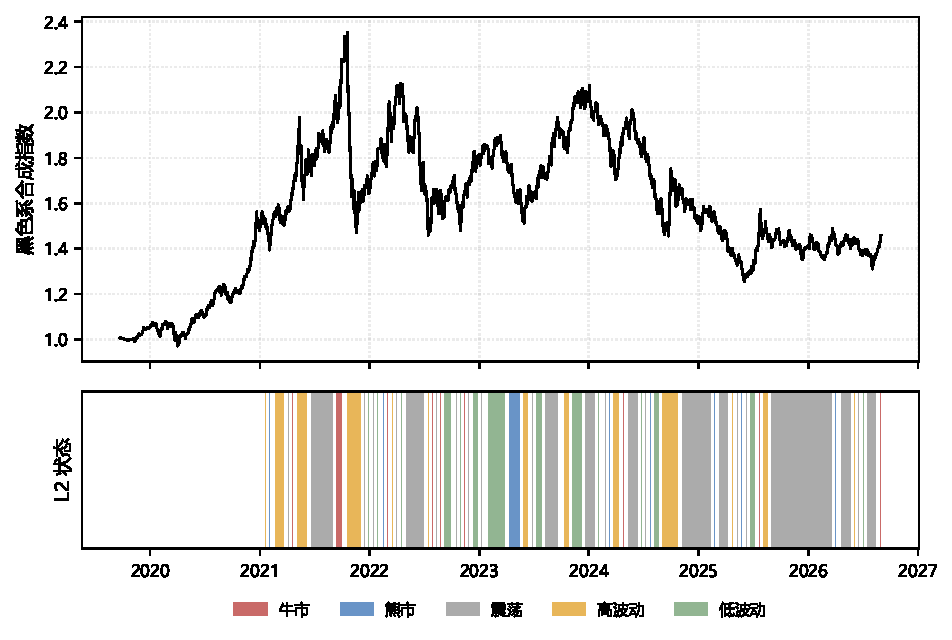
\includegraphics[width=\linewidth]{figures/fig_l2_evolution.pdf}
\caption{黑色系产业链 L2 状态演化（walk-forward 回看，每 10 个交易日重估；色带为状态，上图为合成指数）}
\label{fig:l2-evolution}
\end{figure}

\subsection{案例二：切换统计与检测粒度}

多次回看的区间折叠后得到 68 个状态区间、67 次切换（六年样本，平均约每 37 个自然日一次切换）。各状态的画像与持续期结构如表~\ref{tab:l2-stats} 与图~\ref{fig:l2-stats} 所示。

\begin{table}[htbp]
\centering
\footnotesize
\begin{tabular}{lccccc}
\toprule
\textbf{状态} & \textbf{占比} & \textbf{平均持续期（天）} & \textbf{最长（天）} & \textbf{区间数} & \textbf{平均置信度} \\
\midrule
震荡 & 47.4\% & 25.4 & 200 & 24 & 0.70 \\
高波动 & 19.7\% & 15.9 & 51 & 13 & 0.69 \\
低波动 & 18.2\% & 11.2 & 56 & 14 & 0.65 \\
熊市 & 7.3\% & 4.1 & 33 & 8 & 0.53 \\
牛市 & 7.3\% & 1.8 & 16 & 9 & 0.55 \\
\bottomrule
\end{tabular}
\caption{黑色系 L2 状态画像（2019-11 至 2026-08，137 个决策步）}
\label{tab:l2-stats}
\end{table}

\begin{figure}[htbp]
\centering
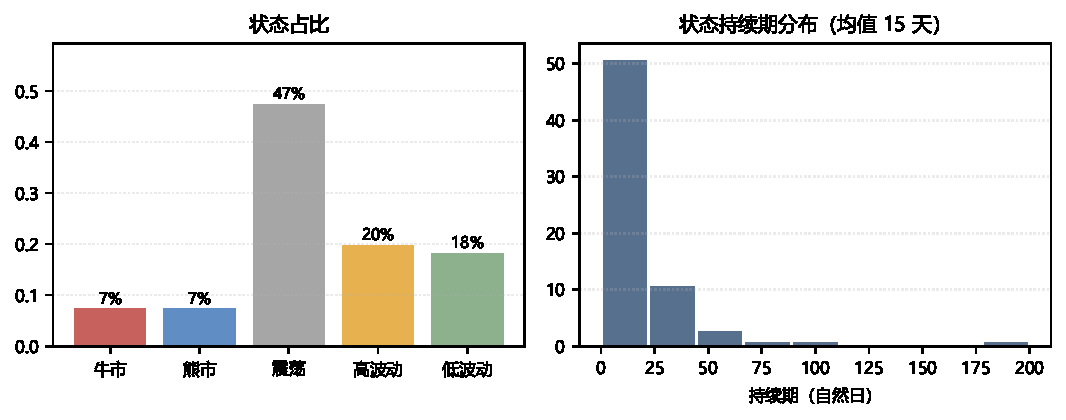
\includegraphics[width=\linewidth]{figures/fig_l2_stats.pdf}
\caption{各状态占比（左）与状态持续期分布（右）}
\label{fig:l2-stats}
\end{figure}

三个值得诚实讨论的发现：

\begin{enumerate}[itemsep=3pt]
\item \textbf{牛/熊是“短促状态”，震荡/波动是常态}。牛市平均仅持续 1.8 个自然日、熊市 4.1 天，而震荡 25.4 天——黑色系在样本期内大部分时间并不存在可持续的“方向性状态”。这直接呼应第一部分的信息论下界：\emph{持续期越短的状态，与噪声在统计上越难区分}；识别器对牛/熊判定给出的平均置信度（$0.53$/$0.55$）也确实低于震荡/高波（$0.65$--$0.70$）——系统的输出与状态的统计现实是自洽的。
\item \textbf{切换频率不低}。六年 67 次切换、年化换手 6.6 倍（条件化口径），说明该系统的自然工作点偏向“敏感”一侧。对成本高度敏感的场景，应把阈值/确认机制向“迟钝”方向调整——这正是第一部分“工作点选择”的工程含义。
\item \textbf{量化延迟的构成}。探到的每个切换时点都包含三层延迟：数据层面（日线收盘可见）、识别层面（HMM 窗口投票的确认）、粒度层面（实证为 10 个交易日）。生产系统消除第三层后可接近日度分辨率，但前两层由统计下界决定，不可消除。
\end{enumerate}

\subsection{案例三：条件化口径与静态口径}

用状态序列驱动一个演示性暴露规则（牛市 $+1$、低波动 $+0.5$、震荡/高波动 $0$、熊市 $-1$；$t$ 日决策、$t+1$ 日生效；单边成本 5\,bps），与买入持有对比，结果如表~\ref{tab:l2-conditional} 与图~\ref{fig:l2-conditional}。

\begin{table}[htbp]
\centering
\footnotesize
\begin{tabular}{lcccccc}
\toprule
\textbf{口径} & \textbf{累计收益} & \textbf{年化收益} & \textbf{年化波动} & \textbf{Sharpe} & \textbf{最大回撤} & \textbf{年换手} \\
\midrule
状态条件化 & 45.0\% & 6.4\% & 11.0\% & 0.56 & $-18.3\%$ & 6.6$\times$ \\
买入持有 & 44.9\% & 8.6\% & 23.3\% & 0.35 & $-46.7\%$ & 0$\times$ \\
\bottomrule
\end{tabular}
\caption{条件化口径与买入持有的对比（演示设定：1 日延迟、单边 5\,bps）}
\label{tab:l2-conditional}
\end{table}

\begin{figure}[htbp]
\centering
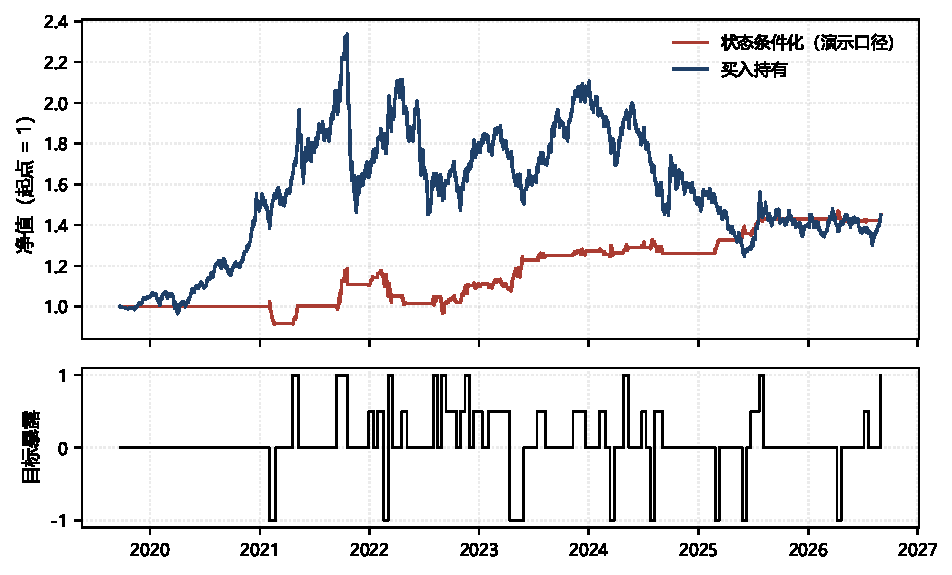
\includegraphics[width=\linewidth]{figures/fig_l2_conditional.pdf}
\caption{条件化口径与买入持有的净值曲线（上）与目标暴露（下，阶梯线）}
\label{fig:l2-conditional}
\end{figure}

结果给出的最重要事实，恰恰\textbf{不是}“条件化跑赢了”，而是：

\begin{itemize}[itemsep=2pt]
\item \textbf{收益中枢几乎不变}（累计 45.0\% vs 44.9\%）——条件化没有、也不应该被期待“创造收益”；
\item \textbf{风险特征近对折}：年化波动率 23.3\% $\to$ 11.0\%，最大回撤 $-46.7\%$ $\to$ $-18.3\%$，Sharpe 从 0.35 提升到 0.56；
\item \textbf{代价是换手}：6.6 倍年换手意味着在更高成本假设（如 15--20\,bps 单边）或流动性约束下，优势会被显著侵蚀——把成本敏感性测试列为必做项，而非可选。
\end{itemize}

这个形态（\emph{收益持平、风险减半}）与第五部分对前沿文献的批判性综合（“价值在风险特征与实施稳健性”）完全一致，是理论与实证之间最有力的交叉验证。

\subsection{发现的诚实汇总}

把三个案例放回理论框架，得到三处呼应，以及必须同时声明的边界：

\begin{enumerate}[itemsep=3pt]
\item \textbf{呼应一（价值定位）}：条件化未提升收益中枢，却在波动与回撤上取得近似减半的改善——系统价值位于风险端。这与信息论下界一致：识别无法“看得更远”，但足以“守得更稳”。
\item \textbf{呼应二（下界现实）}：牛/熊状态的短促持续期与较低置信度，是状态本身接近统计不可检测的直接体现；系统的保守判定（多窗口投票）是对这一现实的正确工程响应。
\item \textbf{呼应三（成本与工作点）}：67 次切换与 6.6$\times$ 换手提示当前工作点偏敏感；面向成本敏感场景，应向“确认更慢、误报更少”方向调整，并接受由此增大的检测延迟。
\item \textbf{边界声明}：本实证覆盖\emph{单一产业链、单一样本区间}（含疫情、地产周期等特殊结构），条件化暴露为\emph{演示性映射}而非策略推荐；结论的效度限于“方法论流程可复现、理论判断可被数据呼应”这两层，不外推为策略有效性证明。
\end{enumerate}
% ============================================================
%  第七部分：诚实的边界与修正判断
% ============================================================

\section{诚实的边界：反方证据与修正判断}
\label{sec:boundaries}

前面的章节建立了方法、验证与工程体系。作为教程的收束，本章必须完成一件很多教程回避的工作：\textbf{系统性地呈现反方证据}——Regime 建模在什么条件下失效、被高估、甚至有害。这不是谦虚的姿态，而是第一部分“信息论下界”与第三部分“验证体系”的必然延伸：一个承认滞后下界的框架，也必须承认自身价值的边界。

\subsection{五条反方证据}

\subsubsection{证据一：拥挤与衰减}

任何被广泛使用的信号都会衰减，Regime 信号不例外。当“状态切换”成为行业共识时，切换时点本身会成为交易对象：防御状态的确认信号被抢先交易，切换的一致性放大流动性冲击——这本质上是第一类非平稳（结构演化）在 Regime 系统自身的投影。更一般地，Harvey et al.~\cite{harvey2016} 关于金融研究中数据窥探的系统性证据提醒我们：\emph{从大量试验中筛选出的“有效模式”，其样本外价值通常远低于样本内读数}。Regime 系统若经过大量窗口/状态数/阈值的筛选，其“有效”结论必须按同一标准折价。

\subsubsection{证据二：样本内解释力 \texorpdfstring{$\ne$}{不等于} 预测力}

HMM 能对历史给出漂亮的状态划分，这几乎不构成证据：任何有足够状态数的模型都能“解释”历史。真正的判据是第三部分的三角验证（模型自洽、结构稳定、经济价值），且经济价值必须在\emph{严格因果}的条件下度量。大量研究报告的 Regime 回测恰恰在这一点上失守（平滑泄漏、全样本参数、缺延迟）——这不是个别错误，而是跨文献的系统性方法论缺陷。

\subsubsection{证据三：状态数的不可辨识}

第二部分已论证：$K$ 的选择是决策分辨率的选择，不是对“真实状态数”的逼近；信息准则常在 $K=2\sim3$ 后改善微弱，而经济可解释性与切换成本往往给出更硬的约束。任何声称“市场确实有 5 个状态”的论述都是过度解读；正确的表述是“在可承受的切换成本下，5 个状态提供了足够的分辨率”。

\subsubsection{证据四：结构演化的持续侵蚀}

第一章把非平稳分成三层：参数漂移、状态切换、结构演化。前两层是 Regime 建模的作用域，第三层不是——它没有可重演的样本。市场微观结构变革、参与者结构变化（被动化、量化渗透率上升）、监管框架调整，会缓慢改变每个状态的统计画像本身。一个在 2016--2020 年训练的“高波动状态”画像，在 2024 年可能已经指向不同的资产行为。这不是模型的失败，而是作用域的边界；应对方式只能是监控（画像漂移检测）与定期重校准，而不是期望一个模型一劳永逸。

\subsubsection{证据五：诊断能力的脆弱性}

无标签世界里的评估依赖间接证据，而间接证据可以被“表演”：优化到漂亮的画像（过拟合状态边界）、在历史上选出最平滑的窗口组合（选择偏差）、用泄漏版回测展示优越性（有意或无意的）。第三部分的检查清单之所以必要，正是因为\textbf{这些表演在表面上与真本事无法区分}——只有通过对照实验（合规版 vs 泄漏版）、扰动检验与多重检验折扣，才能让两者重新可分。

\subsection{修正后的判断：这个系统到底值得做吗}

把全部证据合起来，得到一个修正后的价值定位：

\begin{enumerate}[itemsep=3pt]
\item \textbf{Regime 系统不是预测机器}。它不承诺“更早看到未来”，第一部分的下界论证排除了这种可能性。任何以“提高预测精度”为卖点推销 Regime 建模的论述都应当被怀疑。
\item \textbf{它的真实价值有三层}：
\begin{itemize}[itemsep=2pt]
\item \emph{风险管理的纪律化}：把“什么时候该缩小暴露”从情绪判断变成程序判断（Schwert 的波动率时代、Scherer 的传染证据都指向“防御的价值主要在风险端”）；
\item \emph{策略调度的结构化}：因子权重、杠杆上限、止损参数随状态条件化（第~\ref{sec:strategy}~节的证据：条件化配置显著改善风险调整表现）；
\item \emph{沟通与复盘的语言}：把“最近很难做”翻译为“转折点密度上升、趋势结构恶化”——可量化、可跟踪、可追责。
\end{itemize}
\item \textbf{期望值的诚实锚点}：现有文献的一致信号是\emph{风险特征改善}（波动率、回撤、Calmar）与\emph{实施稳健性}（换手、延迟鲁棒性），而不是收益中枢的抬升。以此为期望值做投入产出评估；若团队的目标是“找到更强的预测信号”，Regime 建模是错误的工具。
\item \textbf{明确的适用边界}：
\begin{itemize}[itemsep=2pt]
\item 适合：资产配置层的姿态与风险预算、多策略资金分配、风控熔断、研究框架与复盘语言；
\item 慎用：作为独立 alpha 信号、日内级别的高频择时、缺少成本约束下的高频状态切换；
\item 禁用场景：以平滑概率做实时决策、以全样本参数做历史回测、以单次样本内结果做资本承诺。
\end{itemize}
\end{enumerate}

\subsection{生产纪律清单（十二条）}

作为全教程的操作性收束，以下清单可直接用于团队审查：

\begin{enumerate}[itemsep=2.5pt]
\item 状态判定只使用\emph{滤波}概率；平滑与离线方法只用于研究与复盘；
\item 参数估计使用滚动/扩展窗口逐步重估，禁止全样本参数进入历史回测；
\item 每一期报告\emph{状态画像}（统计签名）而非状态编号；
\item 状态数 $K$ 的选择同时满足经济可解释性与“肘部法则”，并评估切换成本；
\item 跨窗口追踪状态身份一致性（模板匹配/画像指纹），匹配率骤降即人工复核；
\item 泄漏审计（合规版 vs 泄漏版对照实验）纳入常规回归测试；
\item 稳定性检验（子样本重估、种子扰动、块 bootstrap 区间）常态化输出；
\item 姿态响应不对称：进入防御快、恢复进攻慢；
\item 状态概率连续映射到仓位，避免二值开关；
\item 全部回测计入交易成本与 1--2 期执行延迟；
\item 对多重检验保持折扣意识（显著性的门槛应远高于名义 $t=2$）；
\item 每年做一次结构复核：检测状态画像漂移，决定是否重新校准或降级模型。
\end{enumerate}

\subsection{最后的主句}

\keynote{Regime 系统最诚实的使用方式，是把它当作“风险管理的纪律装置”与“策略调度的语法”，而不是一台预测机器。它能显著改善你“保持姿态”的一致性，但无法让你“看得更远”——它全部的边界与全部的价值，都来自同一个事实。}

\newpage
\appendix
% ============================================================
%  附录
% ============================================================

\section{数学推导补充}

\subsection{EM 算法的单调性证明}

\begin{proposition}[EM 的单调性]
记 $Q(\btheta \mid \btheta') = \E_{S \mid Y, \btheta'}[\log P(Y, S \mid \btheta)]$，则对任意 $\btheta, \btheta'$，
\begin{equation}
\log P(Y \mid \btheta) - \log P(Y \mid \btheta') \;\ge\; Q(\btheta \mid \btheta') - Q(\btheta' \mid \btheta').
\end{equation}
因而 EM 每次迭代（$\btheta_{\text{new}} = \arg\max_{\btheta} Q(\btheta \mid \btheta_{\text{old}})$）后对数似然单调不减。
\end{proposition}

\begin{proof}
从观测似然的条件期望展开开始：
\begin{align}
\log P(Y \mid \btheta) - \log P(Y \mid \btheta')
&= \log \sum_{s} P(Y, s \mid \btheta) - \log P(Y \mid \btheta') \notag \\
&= \log \sum_{s} P(s \mid Y, \btheta')\, \frac{P(Y, s \mid \btheta)}{P(s \mid Y, \btheta')} - \log P(Y \mid \btheta').
\end{align}
对第一项使用 Jensen 不等式（$\log$ 为凹函数）：
\begin{equation}
\ge\; \sum_{s} P(s \mid Y, \btheta')\, \log \frac{P(Y, s \mid \btheta)}{P(s \mid Y, \btheta')} - \log P(Y \mid \btheta').
\end{equation}
把 log 内的分数拆开并整理（注意 $\sum_s P(s \mid Y, \btheta') = 1$）：
\begin{align}
&= \underbrace{\sum_{s} P(s \mid Y, \btheta')\, \log P(Y, s \mid \btheta)}_{=\, Q(\btheta \mid \btheta')}
- \underbrace{\sum_{s} P(s \mid Y, \btheta')\, \log P(Y, s \mid \btheta')}_{=\, Q(\btheta' \mid \btheta')} \notag \\
&= Q(\btheta \mid \btheta') - Q(\btheta' \mid \btheta'),
\end{align}
其中最后一步用了恒等式 $P(s \mid Y, \btheta')\, P(Y \mid \btheta') = P(Y, s \mid \btheta')$（贝叶斯公式），使两个带 $P(Y \mid \btheta')$ 的项相互抵消。因此当 $Q(\btheta \mid \btheta') \ge Q(\btheta' \mid \btheta')$ 时必有 $\log P(Y \mid \btheta) \ge \log P(Y \mid \btheta')$。
\end{proof}

\begin{remark}
这个证明只用到 Jensen 不等式与贝叶斯公式，不依赖任何分布形式——它适用于 HMM、GMM 及一切 EM 估计场景，是附录中唯一需要逐行记住的推导。
\end{remark}

\subsection{前向算法的缩放（scaling）版本}

$\alpha_t(j)$ 随 $t$ 指数衰减，直接计算在 $T$ 稍大时即下溢。标准缩放算法每步归一化：
\begin{align}
\hat\alpha_1(j) &= \pi_j f_j(Y_1) / c_1, \qquad c_1 = \sum_j \pi_j f_j(Y_1), \\
\hat\alpha_t(j) &= \Big[\sum_i \hat\alpha_{t-1}(i)\, a_{ij}\Big] f_j(Y_t) \Big/ c_t, \qquad
c_t = \sum_j \Big[\sum_i \hat\alpha_{t-1}(i) a_{ij}\Big] f_j(Y_t),
\end{align}
其中 $\hat\alpha_t$ 每步之和恒为 $1$。观测对数似然由缩放因子累加恢复：
\begin{equation}
\log P(Y_{1:T} \mid \btheta) \;=\; \sum_{t=1}^{T} \log c_t .
\end{equation}
该恒等式是 Baum--Welch 数值实现中“似然从哪来”的标准答案，也是判断实现正确性的首个自检点（对上式应等于直接计算的小样本似然）。

\subsection{Viterbi 路径与逐点最优的差异}

\begin{example}
设 $K=2$、$T=3$，平滑后验为 $\gamma_1 = (0.6, 0.4)$、$\gamma_2 = (0.6, 0.4)$、$\gamma_3 = (0.6, 0.4)$，而转移矩阵强烈偏好状态稳定（$a_{11} = a_{22} = 0.95$）。逐点最优序列为 $(1,1,1)$；若联合概率最高的路径是 $(2,2,2)$（例如状态 2 的发射似然在三个时点联合占优），则 Viterbi 返回 $(2,2,2)$。两者都不“错误”——它们优化的是不同的目标函数（边缘 vs 联合）；工程含义不同（风险预算 vs 叙事复盘），因此接口必须显式区分。
\end{example}

\subsection{式~\texorpdfstring{\eqref{eq:delay}}{\ref{eq:delay}} 的 Wald 恒等式来源}

对 SPRT，记 $N$ 为停止时刻、$L_N$ 为停止时的累积对数似然比。Wald 恒等式给出
\begin{equation}
\E_{P_1}[L_N] \;=\; \E_{P_1}[N] \cdot \E_{P_1}[\log (p_1/p_0)(Y)],
\end{equation}
当忽略“过冲”时 $\E[L_N] \approx b \approx \log(1/\alpha)$，于是 $\E[N] \approx \log(1/\alpha)/D$。对 CUSUM，将其视为“对每个可能的切换起点重启的 SPRT”即得延迟 $\propto \log(\mathrm{ARL}_0)/D$ 的量级关系。\emph{过冲修正与多状态推广的技术细节超出本教程范围}，但量级结构（延迟与误报的对数交换）在此推广下保持。

\section{术语表}

\begin{longtable}{>{\raggedright\arraybackslash}p{3.0cm}>{\raggedright\arraybackslash}p{8.8cm}}
\toprule
\textbf{术语} & \textbf{含义} \\
\midrule
\endhead
Regime / 状态 & 市场的隐性的、可持久的统计行为模式（如牛/熊、高波/低波、趋势/震荡） \\
滤波（filtering） & $\Prob(S_t = k \mid Y_{1:t})$：只用当前与历史信息推断状态（实时决策唯一合法输入） \\
平滑（smoothing） & $\Prob(S_t = k \mid Y_{1:T})$：使用全样本信息，仅可用于研究复盘 \\
预测（prediction） & $\Prob(S_{t+h} = j \mid Y_{1:t})$：对未来状态的推断 \\
发射分布 & 给定隐状态下观测的条件分布 $F_k$ \\
转移矩阵 $A$ & $a_{ij} = \Prob(S_t = j \mid S_{t-1} = i)$，行和为 1 \\
Label switching & 状态编号的置换不变性：编号无语义，画像才有 \\
状态画像 & 状态的统计签名（均值、波动、持续期等），用于身份追踪 \\
Baum--Welch & HMM 的 EM 学习算法（前向—后向 $+$ 加权统计） \\
Viterbi 解码 & 求联合概率最大的状态\emph{路径}（$\ne$ 逐点最优） \\
MS-GARCH & 波动率方程随状态切换的 Markov-Switching 模型 \\
HSMM & 隐半马尔可夫模型：显式状态时长分布（非几何） \\
跳变惩罚 & 统计跳变模型中惩罚状态切换的 $\lambda$（$0$ 时退化为 K-means） \\
Wasserstein 距离 & 分布间的最优传输距离；用于跨窗口的状态身份对齐 \\
CUSUM & 累积和在线变点检测（Page 1954），阈值控制延迟—误报工作点 \\
BOCPD & 贝叶斯在线变点检测：维护游程长度（run length）后验 \\
游程（run length） & 距最近一次变点的期数（BOCPD 的核心变量） \\
hazard 率 & 每期发生变点的先验概率（几何 hazard 对应期望段长 $1/\lambda$） \\
ARI & 调整后兰德指数：两次分割的一致性度量（稳定性检验用） \\
前瞻偏差 & 回测中使用了当时不可得的信息（平滑/参数/特征/执行四类） \\
工作点 & 延迟—误报前沿上选定的操作点（阈值、确认期、投票规则） \\
条件化先验 & 用高分辨率状态（如产业链）修正低分辨率状态（如品种）的启发式贝叶斯 \\
约束式接口 & 上游输出参数边界（上限/倍率）而非具体仓位，提高对识别误差的容错 \\
\bottomrule
\end{longtable}

\newpage
\printbibliography[title={参考文献}]

\end{document}